\documentclass[11pt]{article}

\usepackage{geometry}
\usepackage[T1]{fontenc}
\usepackage[utf8]{inputenc}
\usepackage{lmodern}
\usepackage{amsmath,amssymb,amsthm,amsfonts}
\usepackage{booktabs}
\usepackage{graphicx}
\usepackage{siunitx}
\usepackage[numbers]{natbib}
\usepackage{hyperref}
\usepackage[nameinlink,noabbrev]{cleveref}
\usepackage{setspace}
\usepackage{subcaption}
\usepackage{placeins}
\geometry{a4paper,margin=2.5cm}
\usepackage{changepage}
\usepackage[normalem]{ulem}
\usepackage{authblk}
\usepackage{array}
\usepackage[table]{xcolor}
\usepackage{tabularx}
\usepackage{tikz}
\usetikzlibrary{arrows.meta,positioning,plotmarks}
\InputIfFileExists{generated/spoofing_empirical_macros.tex}{}{}

\onehalfspacing
\clubpenalty=10000
\widowpenalty=10000
\brokenpenalty=10000
\hypersetup{
    colorlinks=true,
    linkcolor=blue,
    citecolor=blue,
    urlcolor=blue,
    pdftitle={Execution-Conditioned Liquidity Withdrawal and Spoofing-Compatible Sequences},
    pdfauthor={Daniele Maria Di Nosse, Francesco Gigante, Antonio Russo, Fabrizio Lillo}
}


\title{Execution-Conditioned Liquidity Withdrawal and Spoofing-Compatible Sequences}
\author[1]{Daniele Maria Di Nosse\textsuperscript{\dag}}
\author[2]{Francesco Gigante}
\author[2]{Antonio Russo}
\author[1]{Fabrizio Lillo}

\affil[1]{Scuola Normale Superiore, Pisa, Italy}
\affil[2]{Consob, Rome, Italy}
\date{\today}

\begin{document}

\maketitle
\begin{center}
  \footnotesize
  \dag Corresponding author. Email: \texttt{daniele.dinosse@sns.it}
\end{center}

\begin{abstract}
Frequent cancellation is difficult to interpret because both liquidity providers and manipulators can withdraw orders rapidly. We examine a sequence central to the hypothesized spoofing strategy: a participant displays liquidity, executes on the opposite side, and then cancels the displayed orders. Using participant-level messages covering 48,481 executions in Ferrari, Nexi, and Risanamento, we reconstruct the visible limit order book and follow individual orders through this sequence. A continuous score summarizes withdrawal relative to the displayed and executed quantities, with greater weight for earlier cancellation. We examine the accompanying midprice movements separately.

Higher withdrawal scores do not consistently identify the price pattern expected under the hypothesized spoofing strategy. Among executions followed by withdrawal, the score largely reflects the cancelled quantity relative to the executed quantity. Higher scores do not uniformly accompany more favorable price movements. A separate episode-level selection identifies cases in which withdrawal and the required price signs occur together. Replacement orders can also leave displayed liquidity unchanged despite large gross cancellations. Separate timing comparisons find cancellation activity concentrated around execution in Ferrari and Nexi, but not uniformly in Risanamento. The results support reviewing withdrawal, the remaining book, and price movements together. They do not establish manipulative intent or causal price effects, and independently adjudicated manipulation labels are unavailable for validation.
\end{abstract}

\paragraph{Keywords.}
Spoofing detection; market manipulation; limit order book; high-frequency trading; anomaly detection; market maker; market microstructure

\section{Introduction}
\label{sec:introduction}
In an electronic continuous double auction, the limit order book (LOB) shows the visible buy and sell orders waiting to execute. Each new order, amendment, execution, or cancellation changes that book. Algorithmic and high-frequency trading make these changes faster and can improve short-term liquidity. But speed also makes the sequence of actions harder to interpret: a large displayed position may appear and disappear before an observer can assess what happened between its placement and withdrawal.

The hypothesized spoofing strategy uses displayed liquidity to improve an execution on the opposite side. Consider a participant who wants to sell. The participant first displays large bid orders that are not intended to execute. Other traders may interpret the added bid depth as buying pressure and raise their quotes. The participant can then sell at a more favorable price and cancel the bids. Reversing the sides gives the corresponding strategy for a purchase. The Market Abuse Regulation (MAR) prohibits orders and behavior that create false or misleading signals about the supply of, demand for, or price of a financial instrument \cite{EU5962014}.

The difficulty is that each observable action also occurs in legitimate trading. Liquidity providers cancel and replace orders to update prices, control inventory, or avoid trading against better-informed participants. They can therefore generate many cancellations and high order-to-trade ratios without trying to mislead anyone. Order size and cancellation frequency alone do not resolve this ambiguity. Rules based only on these quantities can produce false positives and cannot establish intent.

We therefore ask how the actions fit together, rather than how often cancellation occurs. Was liquidity displayed before the same participant traded on the other side? Did the participant withdraw those orders soon afterward? How much was withdrawn relative to the execution, and did the price follow the directions suggested by the strategy? Participant-level messages let us follow the same orders through these stages. Aggregate activity alone cannot establish that connection.

An execution is the starting point of our reconstruction. For its participant, we identify recent orders still resting on the opposite side and follow their subsequent cancellations. The execution may be passive or aggressive. Because several executions can occur while the same orders remain displayed, we group executions sharing those orders and count each physical cancellation only once. We attribute activity to the original client code where available and to the firm identifier otherwise. These two observation levels remain distinct.

Our first task is to measure withdrawal. We compare the attributed cancelled quantity with both the displayed candidate quantity and the executed quantity. A continuous score combines these comparisons with cancellation delay and orders executions for review. This score describes gross cancellation: it does not subtract newly submitted or replacement orders. We therefore also follow the participant's complete resting profile. That separate measurement shows whether cancellation of recent orders accompanies a decrease in the liquidity still displayed.

Our second task is to examine the associated price path. We measure the price movement from candidate placement to execution, the execution price relative to the placement benchmark, and the movement after cancellation. These quantities do not enter the withdrawal score. We then select a restricted set of episodes in which rapid withdrawal exceeds total executed quantity and the midprice shows both favorable movement before execution and positive reversion after cancellation. This joint selection asks whether a complete hypothesized sequence is observed; it does not define withdrawal itself.

Across the three samples, the withdrawal score largely orders executions by the amount withdrawn relative to the amount traded. Higher scores do not consistently correspond to more favorable price movements. Nor do they necessarily imply a contraction of the participant's complete resting profile. The highest scores can lie outside the restricted set of complete sequences. A separate timing comparison finds cancellation activity concentrated around execution in Ferrari and Nexi, but not in every Risanamento stratum. These results characterize observable behavior. They do not identify intent, causal price effects, or spoofing prevalence.

The economic contrast between market making and spoofing explains why the sequence matters. After reviewing related approaches and the data, we develop two complementary measurements: the evolution of the complete resting profile and the withdrawal of particular recent orders. We then introduce the price diagnostics and explain how executions are grouped into episodes. The results follow the same questions: what is observed, how withdrawal varies, whether it accompanies the expected price path, and how timing and alternative specifications affect the interpretation.

\section{Market Making Versus Spoofing}
\label{sec:mm_vs_spoofing}
Why might a participant display liquidity and then withdraw it after trading on the other side? Market making and spoofing offer different stylized answers. Both can generate frequent cancellations, but the displayed orders serve different economic purposes. We use this contrast to motivate observable measurements, not to assume that every market maker quotes symmetrically or that every spoofing episode follows one pattern.

\subsection{The Market Maker's Problem}
\label{subsec:market_maker}
A market maker supplies liquidity by posting resting orders on the bid and ask sides of the book. In a stylized
inventory-risk benchmark, the dealer seeks to earn the bid--ask spread while controlling inventory risk and exposure to
adverse selection. Optimal quotes therefore depend on both order-arrival rates and the dealer's inventory.

Stochastic-control models often express the dealer's choice through a Hamilton--Jacobi--Bellman equation. The quotes balance execution revenue against inventory risk. A dealer with a long inventory, for example, is exposed to a price decline. Lowering the ask encourages other traders to buy from the dealer, while lowering the bid discourages further sales to the dealer. Both changes help reduce inventory. The chosen adjustment depends on the midprice, the spread needed for compensation, and the penalty for departing from the inventory target.

Cancellation is therefore part of risk management in this benchmark. The dealer removes and reposts quotes when the midprice, inventory, or adverse-selection risk changes. A two-sided presence near the top of the book is the stylized reference, but actual quoting may become asymmetric as conditions change. The benchmark's expected gain comes mainly from earning the spread, rather than deliberately moving the midprice in a chosen direction.

\subsection{The Spoofer's Problem}
\label{subsec:spoofing}
In the spoofing benchmark, displayed liquidity instead serves a hypothesized directional purpose. The participant shows a large order on one side and seeks to execute a smaller order on the other. Traders or algorithms using bid--ask volume imbalance may interpret the large order as short-term price pressure. If they adjust their quotes or trades in response, the resulting movement could improve the participant's opposite-side execution.

The strategy faces a trade-off: the displayed order must be visible, but executing it would create unwanted exposure. An order at the best quote is prominent and relatively exposed to execution. An order at Level 2, Level 3, or deeper has a buffer against immediate execution, while remaining visible in multilevel book data. The hypothesized strategy may therefore spread the displayed quantity across deeper levels instead of placing it all at the touch.

Once the smaller order has executed, the hypothesized purpose of the large display has been fulfilled. Rapid withdrawal would then reduce its remaining execution exposure. This ordering motivates our measurement: we ask whether withdrawal follows an opposite-side execution, rather than measuring cancellation frequency alone. Ordinary quote updates can also follow changes in inventory, fair value, or adverse-selection risk. \Cref{tab:surveillance-models} summarizes the contrasting benchmarks; the records do not directly reveal their motives.

\begin{table}[htbp]
\centering
\caption{Stylized differences used to construct the surveillance diagnostics. These differences describe economic
benchmarks, not observed intent or necessary conditions for either activity.}
\label{tab:surveillance-models}
\renewcommand{\arraystretch}{1.4}
\setlength{\tabcolsep}{8pt}
\rowcolors{2}{gray!4}{white}

\begin{tabularx}{\textwidth}{
    >{\raggedright\arraybackslash\bfseries}p{0.25\textwidth}
    >{\raggedright\arraybackslash}X
    >{\raggedright\arraybackslash}X
}
\toprule
\rowcolor{gray!15}
\textbf{Microstructure Feature} & \textbf{Legitimate Market Maker} & \textbf{Hypothesized Spoofing-Compatible Mechanism} \\
\midrule
Primary objective
& Earn the bid--ask spread while controlling inventory and adverse-selection risk.
& Improve a directional execution through a displayed order-book signal. \\

Order-book imbalance
& Usually maintains two-sided liquidity, with asymmetry arising from inventory and risk management.
& A large, short-lived asymmetry forms the candidate posture. \\

Cancellation motive
& Update quotes to track fair value, control inventory, or limit adverse selection.
& Withdrawal after the smaller opposite-side execution is consistent with the mechanism. \\

Posting-distance trade-off
& Quote near the touch to increase execution probability and earn the spread.
& Remain visible while reducing the risk that the displayed posture executes. \\

Source of expected gain
& Spread capture, without intentionally moving the midprice in a chosen direction.
& A potential favorable price change for the smaller order on the opposite side. \\
\bottomrule
\end{tabularx}
\end{table}

\section{Existing Approaches}
\label{sec:existing_approaches}
Existing methods answer different questions because they classify different objects. Rule-based screens reconstruct order sequences. Statistical methods identify unusual order-book states. Sequence and graph models use temporal or relational patterns in the event data. For our question, the key distinction is between recognizing an unusual book and establishing who displayed, traded against, and withdrew particular orders. The families in \cref{fig:method_taxonomy} can overlap in practice.

\begin{figure}[htbp]
    \centering
    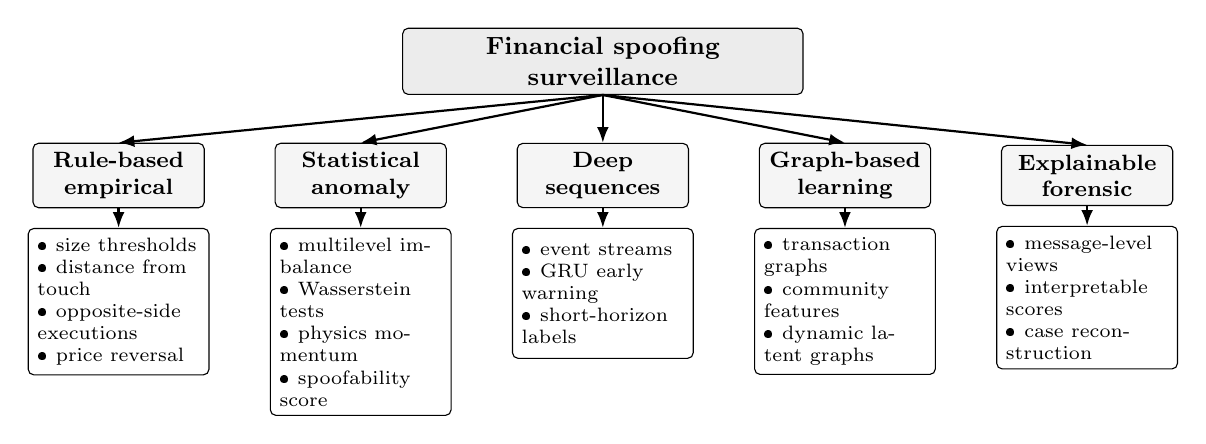
\begin{tikzpicture}[
        font=\scriptsize,
        root/.style={
            draw,
            rounded corners=2pt,
            fill=gray!15,
            align=center,
            text width=0.40\textwidth,
            minimum height=0.8cm,
            font=\small\bfseries
        },
        category/.style={
            draw,
            rounded corners=2pt,
            fill=gray!8,
            align=center,
            text width=0.16\textwidth,
            minimum height=0.75cm,
            font=\footnotesize\bfseries
        },
        detail/.style={
            draw,
            rounded corners=2pt,
            fill=white,
            align=left,
            text width=0.17\textwidth,
            minimum height=1.65cm
        },
        arrow/.style={-{Latex[length=2mm]}, thick}
    ]
        \node[root] (root) at (0,0) {Financial \mbox{spoofing} surveillance};

        \node[category] (rules) at (-6.15,-1.45) {Rule-based\\empirical};
        \node[category] (stat) at (-3.075,-1.45) {Statistical\\anomaly};
        \node[category] (seq) at (0,-1.45) {Deep\\sequences};
        \node[category] (graph) at (3.075,-1.45) {Graph-based\\learning};
        \node[category] (expl) at (6.15,-1.45) {Explainable\\forensic};

        \node[detail, below=0.25cm of rules] (rulesd) {\textbullet\ size thresholds\\\textbullet\ distance from touch\\\textbullet\ opposite-side executions\\\textbullet\ price reversal};
        \node[detail, below=0.25cm of stat] (statd) {\textbullet\ multilevel imbalance\\\textbullet\ Wasserstein tests\\\textbullet\ physics momentum\\\textbullet\ spoofability score};
        \node[detail, below=0.25cm of seq] (seqd) {\textbullet\ event streams\\\textbullet\ GRU early warning\\\textbullet\ short-horizon labels};
        \node[detail, below=0.25cm of graph] (graphd) {\textbullet\ transaction graphs\\\textbullet\ community features\\\textbullet\ dynamic latent graphs};
        \node[detail, below=0.25cm of expl] (expld) {\textbullet\ message-level views\\\textbullet\ interpretable scores\\\textbullet\ case reconstruction};

        \foreach \target in {rules,stat,seq,graph,expl} {
            \draw[arrow] (root.south) -- (\target.north);
        }
        \foreach \source/\target in {rules/rulesd,stat/statd,seq/seqd,graph/graphd,expl/expld} {
            \draw[arrow] (\source.south) -- (\target.north);
        }
    \end{tikzpicture}
    \caption{Method families in the spoofing-detection literature. The categories can overlap; each column identifies
    the main object or representation used by a strand of work.}
    \label{fig:method_taxonomy}
\end{figure}

Rule-based empirical studies are closest to the sequence we reconstruct. Using account-level Korea Exchange data, \cite{LeeEomPark2013} identify large orders away from the best quote, followed by opposite-side trading and withdrawal. Related screens have been applied to Brazilian equities \cite{MendoncaDeGenaro2020}, FX spot markets \cite{StenforsSusai2021}, cross-market FX activity \cite{StenforsEtAl2023}, and Taiwan derivatives \cite{ChenHsiehYang2026}. Their conditions give order size, posting distance, cancellation timing, opposite-side execution, and short-lived price impact a direct microstructure interpretation. Their thresholds are venue-specific, however, and reconstructing the sequence can require privileged message data or account identifiers.

Statistical approaches instead ask whether the book exhibits an unusual state or price-related signal. \cite{TaoDayLingDrapeau2022} derive spoofing incentives from multilevel imbalance and propose a Wasserstein-distance statistic for real-time monitoring. \cite{LiPolukarovaVentre2023} model the book as a statistical-physics system and detect abnormal momentum in cryptocurrency markets. Explainable forensic methods partly overlap with these approaches: message-level visualization can reconstruct prosecuted episodes \cite{DebieEtAl2023}, while interpretable probabilistic neural networks assess how an isolated limit order changes the conditional distribution of future prices and the expected gain from a hypothetical manipulation strategy \cite{FabreChallet2025}. This last quantity measures order-level \emph{spoofability}. It does not establish that the same participant generated the displayed posture, opposite-side execution, and withdrawal. We address that complementary attribution question, keeping client and firm observation levels separate.

Machine-learning methods represent connections across time or across traders. \cite{TuccellaNadlerSerban2021} formulate an early-warning task and train a gated recurrent unit model on cryptocurrency order-book event streams. Graph-based methods represent traders and transactions as a network, allowing the model to capture coordinated patterns \cite{KangMuNing2023,KangMuNing2024,XiangEtAl2025}. Reported approaches combine temporal transaction graphs, community features, and dynamic latent representations. Their performance is difficult to compare directly because market settings, available labels, and validation designs differ.

For the present analysis, this literature motivates interpretable measurements tied to identifiable orders. Candidate quantity, posting distance, withdrawal timing, and the opposite-side execution must remain visible in the reconstruction. Evaluation is a separate problem: enforcement labels are scarce and noisy, positive cases are rare, and false positives consume analyst time. With the evidence available here, we retain the inspectability of rule-based surveillance and use the proprietary messages to describe participant-level sequences.

\section{Data}
\label{sec:data}

The empirical question requires messages that connect orders to participants. We use three CONSOB limit-order-book samples: Risanamento covers June--November 2024, Nexi covers 23 April 2024, and Ferrari covers 13 June 2024. Their durations and participant compositions differ. Comparisons across instruments therefore describe these samples rather than isolate an instrument effect.

The messages allow us to reconstruct which orders are visible, who submitted them, and how they change over time.
For each instrument, we reconstruct the book from order-level events and infer the tick size from the best quotes.
We examine the first ten book ranks. Within that view, we distinguish the participant's complete resting liquidity
from the recent opposite-side orders followed around an execution.

Identifying the participant requires care because the original client code is not present on every message.
We use that code when available and the firm identifier only when it is missing. The technical client value
\texttt{0} denotes missing information and therefore also calls for firm attribution where available.
Client and firm identities remain separate: a message identified by client is not merged with one identified only by
firm. Messages missing both identifiers are excluded from this analysis; none occurs in the reported samples.
Firm attribution can pool several clients, so it cannot be interpreted as the history of one economic account.
We retain the attribution level throughout the analysis.

In the model, participant therefore denotes an attribution unit: an original client where identified, or a separately retained firm fallback. It does not always denote a single economic account.

Execution role is a separate property. CONSOB has confirmed the decoding of the passive and aggressive flags used here.
Passive execution means that a resting limit order is filled; aggressive execution means that a market order or a
marketable limit order crosses the spread. In all three samples, paired trade messages carry either one passive and one
aggressive side, or two unassigned sides. We retain messages marked exclusively passive or exclusively aggressive and
exclude those for which both flags are set or both are absent.

A single order may execute through several partial fills. Counting each fill independently would fragment one execution, so we group related messages into an \emph{execution cluster}, hereafter an execution.

The messages must share the participant, order identifier, role, side, and trading partition. A partition is defined by trading date, venue, market, instrument, and the source code for the exchange market mechanism (EMM). Passive fills must also share a resting price; an aggressive order may sweep several traded prices.

The grouping also requires continuity in time and in the order's lifecycle. Consecutive messages must be no more than $100$ milliseconds apart, with no intervening cancellation, modification, or new-order lifecycle event for that order. We do not report sensitivity to this operational gap choice. Original message identifiers and group membership remain available for inspection. Later, executions sharing candidate orders are grouped into episodes, which allow us to count repeated postures within a participant and day.

Timing the sequence requires two source clocks. We use \texttt{SEQUENCETIME}, defined as nanoseconds since the UTC epoch,
to order messages, reconstruct the book, measure order age, and locate cancellations and subsequent book states.
For execution messages, \texttt{TRADETIME} instead supplies the time of trading. We retain integer nanoseconds for
comparisons and do not substitute another field if the required clock is missing. Storage units should not be confused
with observed precision: trade times lie on a $1$-millisecond grid, whereas sequence timestamps have sub-millisecond values.

Comparing an execution with a later cancellation assumes that the two clocks share a timebase. The selected execution
rows align numerically, with trade time preceding sequence time, but the source dictionary does not independently
certify the UTC origin of \texttt{TRADETIME}. We adopt a common timebase for this exploratory analysis; the observed
alignment alone establishes neither a documented timezone nor finer timing precision.

The main specification follows the complete profile over a $10$-second window after execution. Candidate orders may
have been observed for at most $90$ seconds before execution, and a cancellation is attributed only within the
$2$-second rapid-withdrawal window. Price reversion is measured over a separate $2$-second horizon beginning at each
assigned cancellation. The model below explains the role of each interval.

\section{Model}
\label{sec:model}
The economic sequence raises two distinct measurement questions. First, does the participant's displayed profile change after an opposite-side execution? Second, are the particular orders present before that execution cancelled soon afterward? The answers need not agree: replacements may keep the profile unchanged even when the original orders disappear. We therefore follow both the complete profile and individual recent orders. We then compare the withdrawn quantity with the executed quantity and examine the associated price path.

We begin with the complete profile across the top $n$ book levels. It describes how the participant's liquidity is distributed across ranks and between sides. We next fix a set of recent opposite-side orders at execution and follow their cancellations. The first object measures a changing book state; the second records what happens to specific orders. Keeping them separate prevents a change in overall depth from being mistaken for withdrawal of the selected orders.

These measurements also have different roles. The withdrawal score orders individual executions for review. Executions sharing candidate orders are then combined into episodes, on which we apply the stricter quantity and price conditions. A high execution score and membership in a selected episode are therefore not interchangeable.

% \subsection{Spoofer's timeline}
% \label{subsec:spoofing_timeline}
% \begin{enumerate}
%     \item The spoofer posts a large non bona fide order far away from the best quote and, simultaneously, a small bona 
%     fide order close to the best quote
%     \item The spoofer's small order gets executed due to the price move induced by the artificially increased volume
%     on the opposite side of the book
%     \item The spoofer cancels the large non bona fide order immediately after the execution
%     \begin{figure}[htbp]
%     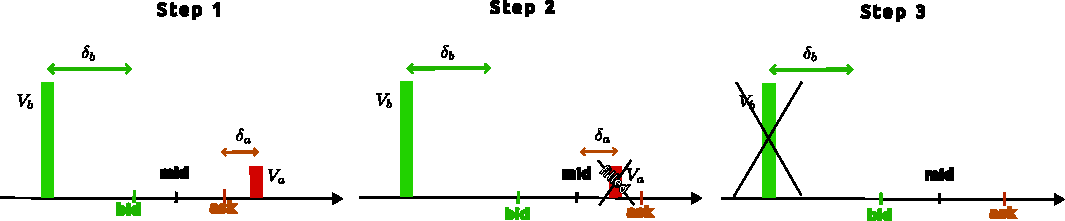
\includegraphics[width=\textwidth]{images/spoofer.pdf}
%     \caption{Timeline of a spoofing episode}
%     \end{figure}

% \end{enumerate}
% Let $i$ indicate the agent of interest, $V_a$ and $V_b$ represent the volumes of the agent's ask and bid orders, 
% respectively, and $\delta_a$ and $\delta_b$ represent their posting distances from the best quote. We consider 
% the following metric that we call distance-weighted imbalance:
% \begin{equation}
%     \left. \text{imb}_{t}^i = \frac{V_a \delta_a - V_b \delta_b}{V_a + V_b} \right|_i
% \end{equation}
% If we consider a sell intent for the spoofer, we expect $\text{imb}_{t}^i$ to be negative at step 1, to become more 
% negative at step 2, and to return to zero at step 3. The opposite holds for a buy intent.
% The crucial point is to distinguish this situation of imbalance between bid and ask from a rebalncing strategy of the market
% maker. In fact, a market maker can also post a large order on one side of the book and a small order on the other side, 
% but in this case we expect the large order to be close to the best quote and the small order to be far from the best 
% quote, while for a spoofer we seek for the opposite. Hence, in this case the imbalance would be positive and it would move
% towards zero more smoothly as the big order is executed, without a sharp and sudden jump as in the spoofer case.

\subsection{A Spatio-Temporal Framework for Spoofing Detection}
\label{sec:spoofer_timeline}

Consider the hypothetical sequence in \cref{fig:topn_spoofing_timeline}. A participant displays large bid orders while a smaller sell order rests near the best ask. The sell order executes, and the participant then cancels the bids. The example makes the sides and ordering explicit; it is not an empirical case. Reversing bid and ask gives the corresponding buy-side sequence.

\begin{figure}[htbp]
    \centering
    \resizebox{0.95\textwidth}{!}{%
    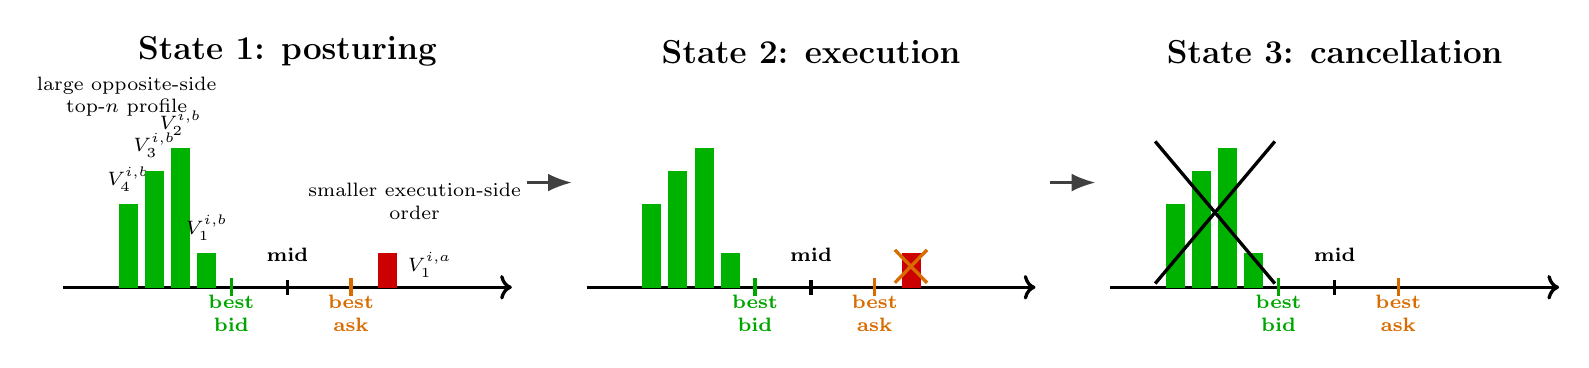
\begin{tikzpicture}[
        x=0.95cm,
        y=0.95cm,
        font=\small,
        book/.style={->, very thick},
        quote/.style={very thick},
        bid/.style={green!65!black},
        ask/.style={orange!85!black},
        fake/.style={fill=green!70!black, draw=green!70!black},
        real/.style={fill=red!80!black, draw=red!80!black},
        layer/.style={draw=black!45, fill=gray!8, rounded corners=2pt, minimum width=0.40cm},
        dist/.style={<->, black!70, very thick}
    ]
        \foreach \xshift/\step in {0/State 1: posturing,7.0/State 2: execution,14.0/State 3: cancellation} {
            \node[font=\large\bfseries] at (\xshift+3.0,3.15) {\step};
            \draw[book] (\xshift,0) -- (\xshift+6.0,0);
            \draw[quote,bid] (\xshift+2.25,-0.12) -- (\xshift+2.25,0.12)
                node[below=0.08cm, align=center, font=\scriptsize\bfseries] {best\\bid};
            \draw[quote] (\xshift+3.00,-0.10) -- (\xshift+3.00,0.10)
                node[above=0.10cm, font=\scriptsize\bfseries] {mid};
            \draw[quote,ask] (\xshift+3.85,-0.12) -- (\xshift+3.85,0.12)
                node[below=0.08cm, align=center, font=\scriptsize\bfseries] {best\\ask};
        }

        % State 1: layered bid-side deceptive profile and small ask-side bona fide order.
        \foreach \x/\h/\lab in {0.75/1.10/{$V^{i,b}_{4}$},1.10/1.55/{$V^{i,b}_{3}$},1.45/1.85/{$V^{i,b}_{2}$},1.80/0.45/{$V^{i,b}_{1}$}} {
            \draw[fake] (\x,0) rectangle +(0.24,\h);
            \node[above, font=\scriptsize] at (\x+0.12,\h+0.05) {\lab};
        }
        \draw[real] (4.22,0) rectangle +(0.24,0.45);
        \node[right, font=\scriptsize] at (4.48,0.30) {$V^{i,a}_{1}$};
        \node[align=center, font=\scriptsize] at (0.85,2.55) {large opposite-side\\top-$n$ profile};
        \node[align=center, font=\scriptsize] at (4.70,1.15) {smaller execution-side\\order};

        % State 2.
        \foreach \x/\h in {7.75/1.10,8.10/1.55,8.45/1.85,8.80/0.45} {
            \draw[fake] (\x,0) rectangle +(0.24,\h);
        }
        \draw[real] (11.22,0) rectangle +(0.24,0.45);
        \draw[orange!85!black, very thick] (11.12,0.06) -- (11.55,0.50);
        \draw[orange!85!black, very thick] (11.55,0.06) -- (11.12,0.50);


        % State 3.
        \foreach \x/\h in {14.75/1.10,15.10/1.55,15.45/1.85,15.80/0.45} {
            \draw[fake] (\x,0) rectangle +(0.24,\h);
        }
        \draw[black, very thick] (14.60,0.05) -- (16.20,1.95);
        \draw[black, very thick] (16.20,0.05) -- (14.60,1.95);


        \draw[-{Latex[length=3mm]}, thick, black!75] (6.2,1.4) -- (6.8,1.4);
        \draw[-{Latex[length=3mm]}, thick, black!75] (13.2,1.4) -- (13.8,1.4);
    \end{tikzpicture}%
    }
    \caption{Schematic top-$n$ timeline for the hypothesized spoofing mechanism. The large candidate posture forms an
    agent-specific depth profile over several bid levels, while the smaller order rests near the opposite best quote. The
    construction applies symmetrically to candidate buy- and sell-intent episodes. The figure shows the passive execution
    route; the operational reconstruction also admits an aggressive execution by the same actor.}
    \label{fig:topn_spoofing_timeline}
\end{figure}
\FloatBarrier

The displayed quantity need not be concentrated in one order at the best quote. It may lie at Level 2, Level 3, or across
adjacent levels, remaining visible while facing less immediate execution risk. For participant $i$, the hypothesized
sequence has three states:
\begin{enumerate}
    \item \textbf{State 1 (Candidate Posturing):} Shortly before execution, the participant displays a large quantity
    on one side, typically away from the touch. We call this arrangement of displayed orders the candidate posture.
    \item \textbf{State 2 (Execution):} A smaller order executes on the opposite side while the large profile is still
    present. Under the hypothesized mechanism, the displayed profile can coincide with a more extreme measured imbalance
    before execution.
    \item \textbf{State 3 (Withdrawal):} The participant rapidly cancels the opposite-side profile. Under the stylized
    mechanism, this timing is consistent with reducing subsequent exposure to execution.
\end{enumerate}

The figure shows a passive execution in State 2; the reconstruction also admits an aggressive one. The execution roles
defined in \cref{sec:data} determine how we group and measure executions, without changing the participant's identity.

The illustration motivates the ordering of events, but does not determine which orders qualify. We therefore need an operational candidate set and a separate rule for assigning subsequent cancellations.

For the candidate set, we select the same participant's opposite-side orders that are active in the top $10$ ranks immediately before the first execution message and were first observed no more than $90$ seconds earlier. The age limit excludes long-lived liquidity. We then look for cancellations that can be attributed within $2$ seconds. The definitions below specify the book ranks, timing, and attribution rule.

Executions sharing candidate orders form an episode under the rule below. At that level, the strict selection additionally requires unique attributed withdrawal to exceed total execution quantity, positive favorable midprice movement, and positive midprice reversion. This episode-level conjunction is distinct from selecting candidate orders or assigning their cancellations.

\subsubsection{\texorpdfstring{Top-$n$}{Top-n} Participant-Specific Depth Profiles}
\label{subsec:topn_depth_profiles}

To describe the complete profile, we retain the quantity at each rank instead of summing it immediately. Let $s\in\{b,a\}$ denote the bid or ask side, and $k=1,\ldots,n$ the book rank, with $k=1$ at that side's best quote. Participant $i$'s displayed volume at time $t$, side $s$, and rank $k$ is $V^{i,s}_{k}(t)$. The depth profile is the vector
\begin{equation}
    \mathbf{V}^{i,s}_{n}(t)
    = \left(V^{i,s}_{1}(t),\ldots,V^{i,s}_{n}(t)\right)
\end{equation}
This vector keeps the quantities at the first $n$ ranks separate. Two profiles can have the same total volume but place it differently
across the book. They need not have the same execution risk, so a single total would lose information relevant to the
hypothesized sequence.

The size of a participant's order also needs a market reference. The same displayed volume represents a different share
of liquidity in a shallow book and a deep one, making raw quantities difficult to compare across assets or intraday
periods. We therefore divide participant volume by total market depth at the same side and rank:
\begin{equation}
    \widetilde V^{i,s}_{k}(t)
    =\begin{cases}
    \dfrac{V^{i,s}_{k}(t)}{D^{s}_{k}(t)},
    & D^{s}_{k}(t)>0,\\
    0,
    & D^{s}_{k}(t)=0,
    \end{cases}
    \label{eq:relative_agent_depth}
\end{equation}
where $D^{s}_{k}(t)$ is total displayed market depth on side $s$ and rank $k$. The instrument index is suppressed in participant-profile formulas; $D^{m,s}_{k}(t)$ below denotes the same market depth for instrument $m$. When that depth is positive,
$\widetilde V^{i,s}_{k}(t)$ is the fraction supplied by participant $i$. When no depth is present, we assign zero to the
relative volume at that rank. This convention does not make an imbalance well-defined when the participant has no
positive weighted liquidity on either side; that case remains undefined.

Rank identifies a level's position in the book, but does not specify its price distance from the best quote. We denote
the distance from the touch by $d^{s}_{k}(t)$ and measure it as the number of ticks between rank $k$ and the same-side best
quote, plus one. The shift gives Rank 1 a positive distance while preserving the ordering of deeper ranks. These
distances provide the starting point for the weighting scheme introduced next.

\subsubsection{Multilevel Distance-Weighted Imbalance}
\label{subsec:multilevel_dwi}

\paragraph{Economic intuition and a stylized parametric benchmark.}
Comparing the two sides requires a way to summarize their rank-by-rank volumes. A simple sum would treat liquidity at the best quote like liquidity deeper in the book. The hypothesized strategy instead involves a trade-off between visibility and exposure to execution. We represent that trade-off by a depth kernel: a set of weights over the first $n$ ranks. A parametric example explains the idea before we define the empirical weights.

In the example, visibility decreases with distance from the touch, while protection from immediate execution increases.
Multiplying these components and normalizing across ranks gives
\begin{equation}
    \omega^{s,\mathrm{par}}_{k}(t)
    =
    \frac{
        e^{-\lambda d^{s}_{k}(t)}
        \left(1-e^{-\kappa d^{s}_{k}(t)}\right)
    }{
        \sum_{\ell=1}^{n}
        e^{-\lambda d^{s}_{\ell}(t)}\left(
        1-e^{-\kappa d^{s}_{\ell}(t)}\right)
    },
    \label{eq:depth_kernel}
\end{equation}
Here $e^{-\lambda d}$ is the visibility component and $1-e^{-\kappa d}$ is the protection component. Their product
gives less weight both to prices exposed to immediate execution and to prices so distant that visibility is low.
The parameters $\lambda$ and $\kappa$ control how quickly the two components change with distance.
\Cref{fig:depth_kernel_behavior} illustrates this balance and the normalization of the resulting weights.

This parametric expression is a conceptual benchmark, not an estimated profile. We do not fit $\lambda$ or $\kappa$ or
use these exponential weights in the empirical results. Instead, we measure the two components separately for each
instrument and book side.

\begin{figure}[htbp]
    \centering
    \resizebox{0.95\textwidth}{!}{%
    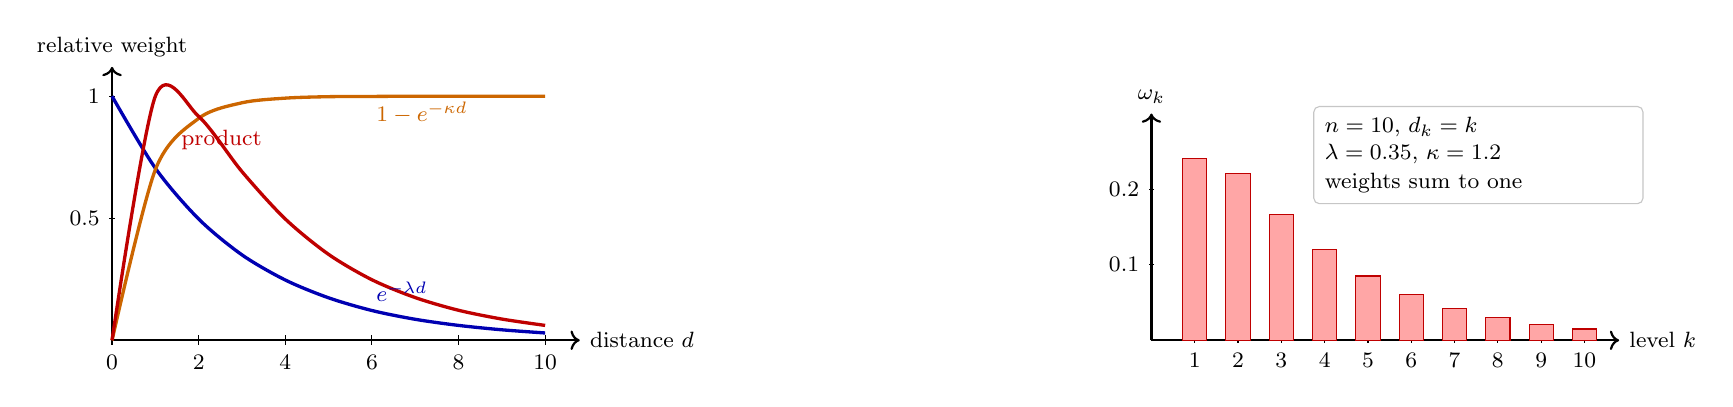
\begin{tikzpicture}[
        x=0.55cm,
        y=3.1cm,
        font=\footnotesize,
        axis/.style={->, thick},
        visibility/.style={very thick, blue!70!black},
        protection/.style={very thick, orange!80!black},
        kernel/.style={very thick, red!75!black},
        weightbar/.style={fill=red!35, draw=red!75!black},
        note/.style={draw=gray!45, rounded corners=2pt, fill=white, align=left, text width=3.9cm, inner sep=4pt}
    ]
        % Left panel: unnormalised ingredients, with the product rescaled to unit peak.
        \draw[axis] (0,0) -- (10.8,0) node[right] {distance $d$};
        \draw[axis] (0,0) -- (0,1.12) node[above, align=center] {relative weight};
        \foreach \x in {0,2,4,6,8,10} {
            \draw (\x,0.02) -- (\x,-0.02) node[below] {\x};
        }
        \foreach \y/\lab in {0.5/$0.5$,1/$1$} {
            \draw (0.06,\y) -- (-0.06,\y) node[left] {\lab};
        }

        \draw[visibility]
            plot[smooth] coordinates {(0,1.000) (1,0.705) (2,0.497) (3,0.350) (4,0.247) (5,0.174) (6,0.122) (7,0.086) (8,0.061) (9,0.043) (10,0.030)};
        \draw[protection]
            plot[smooth] coordinates {(0,0.000) (1,0.699) (2,0.909) (3,0.973) (4,0.992) (5,0.998) (6,0.999) (7,1.000) (8,1.000) (9,1.000) (10,1.000)};
        \draw[kernel]
            plot[smooth] coordinates {(0,0.000) (1,1.000) (2,0.917) (3,0.691) (4,0.497) (5,0.352) (6,0.248) (7,0.175) (8,0.123) (9,0.087) (10,0.061)};
        \node[visibility, anchor=west] at (5.85,0.20) {$e^{-\lambda d}$};
        \node[protection, anchor=west] at (5.85,0.93) {$1-e^{-\kappa d}$};
        \node[kernel, anchor=west] at (1.35,0.82) {product};

        % Right panel: discrete normalised top-n kernel weights.
        \begin{scope}[xshift=13.2cm, y=9.6cm]
            \draw[axis] (0,0) -- (10.8,0) node[right] {level $k$};
            \draw[axis] (0,0) -- (0,0.30) node[above] {$\omega_k$};
            \foreach \x in {1,2,3,4,5,6,7,8,9,10} {
                \draw (\x,0.004) -- (\x,-0.004) node[below] {\x};
            }
            \foreach \y/\lab in {0.1/$0.1$,0.2/$0.2$} {
                \draw (0.06,\y) -- (-0.06,\y) node[left] {\lab};
            }
            \foreach \x/\h in {1/0.241,2/0.221,3/0.166,4/0.120,5/0.085,6/0.060,7/0.042,8/0.030,9/0.021,10/0.015} {
                \draw[weightbar] (\x-0.28,0) rectangle (\x+0.28,\h);
            }
            \node[note] at (7.55,0.245)
            {$n=10$, $d_k=k$\\
            $\lambda=0.35$, $\kappa=1.2$\\[1pt]
            weights sum to one};
        \end{scope}
    \end{tikzpicture}%
    }
    \caption{Conceptual depth kernel in \cref{eq:depth_kernel}. The left panel shows decreasing visibility, increasing
    protection from immediate execution, and their product. The right panel shows normalized weights for one illustrative
    parameter choice. The empirical analysis uses the instrument- and side-specific kernel in
    \cref{eq:empirical_depth_kernel}, not these parametric weights.}
    \label{fig:depth_kernel_behavior}
\end{figure}

\paragraph{Operational empirical depth kernel.}
The empirical kernel assigns weights using two observable properties of each rank. How often does trading reach its displayed price? How strongly does its depth co-move with later midprice changes? We give more weight to ranks that are rarely reached but have stronger price co-movement. Both components are estimated for instrument $m$, side $s$, and rank $k$ over a common horizon $H$. Calibration uses rank, even though its distance from the touch in ticks changes over time.

To estimate exposure, we reconstruct the top-$n$ book after each message. The set $\mathcal{O}_{m,s,k}$ contains snapshots where rank $k$ exists on side $s$ and has positive depth. For each snapshot at $t$, the indicator $I^{m,s}_{t,k}(H)$ equals one if an execution in $(t,t+H]$ reaches or passes the displayed price. Thus an ask price is reached when the maximum execution price is no lower than that price, and a bid price is reached when the minimum execution price is no higher than that price. Averaging the indicator gives the observed hit frequency:
\begin{equation}
    \widehat p^{m,s}_{k}(H)
    =
    \frac{
        \sum_{t\in\mathcal{O}_{m,s,k}}I^{m,s}_{t,k}(H)
    }{
        |\mathcal{O}_{m,s,k}|
    }.
    \label{eq:empirical_hit_probability}
\end{equation}
Each snapshot contributes once to \cref{eq:empirical_hit_probability}, irrespective of the rank's distance from the touch.
We pool hits and exposures rather than average hit rates estimated separately by distance. Tick distances describe the
observations but neither define additional calibration groups nor enter a parametric fit.

A price being reached is not the same as a particular order being filled. Queue position, order size, and intervening cancellations also determine execution. We use the complement of the hit frequency as a descriptive measure of protection from trading:
\begin{equation}
    \widehat\rho^{m,s}_{k}(H)=1-\widehat p^{m,s}_{k}(H),
    \label{eq:empirical_protection_profile}
\end{equation}
A value of $\widehat\rho^{m,s}_{k}(H)$ near one indicates that rank $k$ is rarely reached over horizon $H$.

The second component concerns price co-movement, rather than exposure to trading. We ask whether the market's depth share at a rank is associated with later midprice changes. This uses total market depth, not participant $i$'s orders. Let $D^{m,s}_{k}(t)$ be market depth at side $s$ and rank $k$. Its reference total is the depth across both sides of the top-$n$ book:
\begin{equation}
    D^{m}_{n}(t)
    =
    \sum_{r=1}^{n}\left(D^{m,a}_{r}(t)+D^{m,b}_{r}(t)\right).
    \label{eq:total_topn_market_depth}
\end{equation}
We express each rank's depth as a share of this total, using opposite signs for ask and bid contributions:
\begin{equation}
    Z^{m,s}_{t,k}
    =
    \sigma_s\frac{D^{m,s}_{k}(t)}{D^{m}_{n}(t)},
    \qquad
    \sigma_s= \begin{cases}
        +1, & s=a,\\
        -1, & s=b.
    \end{cases}
    \label{eq:normalized_level_contribution}
\end{equation}
The magnitude $|Z^{m,s}_{t,k}|$ is the fraction of visible top-$n$ depth supplied by that side and rank. The sign makes ask
and bid depth contribute in opposite directions to imbalance.

For each eligible snapshot, we pair the signed depth share with the subsequent price change. Let $M^m_{t,H}$ be the last finite reconstructed midprice after $t$ and no later than $t+H$, and write $\Delta M^m_{t,H}=M^m_{t,H}-M^m(t)$. The set $\mathcal{V}_{m,s,k}(H)$ retains rank-$k$ snapshots with both midprices finite. We measure the magnitude of co-movement by the absolute sample covariance:
\begin{equation}
    \widehat\nu^{m,s}_{k}(H)
    =
    \left|
        \frac{1}{|\mathcal{V}_{m,s,k}(H)|}
        \sum_{t\in\mathcal{V}_{m,s,k}(H)}
        \left(Z^{m,s}_{t,k}-\overline Z^{m,s}_{k}\right)
        \left(\Delta M^m_{t,H}-\overline{\Delta M}^{m,s}_{k,H}\right)
    \right|.
    \label{eq:empirical_visibility_covariance}
\end{equation}
The overbars are sample means over $\mathcal{V}_{m,s,k}(H)$, and the sum is divided by the number of eligible snapshots.
Taking the absolute value retains the magnitude of co-movement, not its direction. As with the hit frequency, we pool
observations across tick distances before estimating the covariance, rather than averaging estimates for separate
distance groups.

The covariance supplies a weight, not an estimate of causal price impact. It is measured in instrument-specific price
units, so we use it to compare ranks on the same side of one instrument, not to compare covariance magnitudes across assets.
Its role corresponds to visibility in the conceptual benchmark, but the observable is price association, not visibility itself. Taking its absolute value also gives the same weight to equally strong positive and negative associations.

We now combine the two components as in \cref{eq:depth_kernel}, replacing the exponential functions with their empirical
proxies. Before multiplying them, we bound protection below by zero and apply a numerical floor of $10^{-12}$ to the
absolute covariance:
\begin{equation}
    \widetilde\rho^{m,s}_{k}(H)=\max\{1-\widehat p^{m,s}_{k}(H),0\},
    \qquad
    \widetilde\nu^{m,s}_{k}(H)=\max\{\widehat\nu^{m,s}_{k}(H),10^{-12}\},
    \label{eq:empirical_kernel_floors}
\end{equation}
We normalize the product of these two quantities within each instrument and side:
\begin{equation}
    \widehat\omega^{m,s}_{k}(H)
    =
    \frac{
        \widetilde\nu^{m,s}_{k}(H)\,\widetilde\rho^{m,s}_{k}(H)
    }{
        \sum_{\ell=1}^{n}\widetilde\nu^{m,s}_{\ell}(H)\,\widetilde\rho^{m,s}_{\ell}(H)
    }.
    \label{eq:empirical_depth_kernel}
\end{equation}
This normalization requires a finite, strictly positive denominator. If all ranks have zero protection, or if the product
is otherwise degenerate, no kernel is reported. Every kernel in \cref{tab:empirical_depth_kernel_calibration} satisfies
this requirement and sums to one before rounding.

The covariance floor is a numerical regularizer. If estimated covariances lie at or below it, protection can largely
determine the relative weights. Such weights should not be read as evidence of differences in price association across ranks.

In the remaining formulas, we use the shorthand
$\omega^{s}_{k}(t)\equiv\widehat\omega^{m,s}_{k}(H)$ for an event in instrument $m$; the time argument indicates that the
fixed weight is applied to a time-varying profile. There is one weight for each $(m,s,k)$ combination, shared by all
participants and events in that instrument. We do not recalibrate it for an individual event or its outcome.
The descriptive analysis uses each instrument's full sample. Prospective use must estimate the kernel on an earlier
training period and hold it fixed to exclude future order flow from the weights.

\begin{table}[htbp]
\centering
\caption{Operational full-sample empirical top-$10$ depth-kernel weights at horizon $H=10$ seconds. Values are rounded to
three decimal places and sum to one within each instrument and side before rounding. These weights, rather than fitted
exponential parameters, enter the empirical spoofing metrics.}
\label{tab:empirical_depth_kernel_calibration}
\scriptsize
\setlength{\tabcolsep}{1.7pt}
\begin{tabular}{ll*{10}{r}}
\toprule
Instrument & Side & $\widehat\omega_1$ & $\widehat\omega_2$ & $\widehat\omega_3$ & $\widehat\omega_4$ & $\widehat\omega_5$ & $\widehat\omega_6$ & $\widehat\omega_7$ & $\widehat\omega_8$ & $\widehat\omega_9$ & $\widehat\omega_{10}$ \\
\midrule
Risanamento & Ask & 0.127 & 0.248 & 0.348 & 0.062 & 0.004 & 0.039 & 0.018 & 0.012 & 0.078 & 0.064 \\
             & Bid & 0.526 & 0.012 & 0.019 & 0.146 & 0.091 & 0.065 & 0.082 & 0.034 & 0.002 & 0.024 \\
Nexi        & Ask & 0.028 & 0.069 & 0.033 & 0.138 & 0.225 & 0.149 & 0.275 & 0.011 & 0.020 & 0.051 \\
             & Bid & 0.045 & 0.166 & 0.184 & 0.276 & 0.165 & 0.033 & 0.006 & 0.052 & 0.064 & 0.008 \\
Ferrari     & Ask & 0.095 & 0.022 & 0.016 & 0.209 & 0.270 & 0.032 & 0.144 & 0.032 & 0.033 & 0.147 \\
             & Bid & 0.148 & 0.107 & 0.007 & 0.054 & 0.072 & 0.197 & 0.102 & 0.038 & 0.176 & 0.100 \\
\bottomrule
\end{tabular}
\end{table}

\FloatBarrier

The operational calibration uses the first ten ranks and the same $H=10$ second horizon for every instrument. It produces
20 weights per instrument, one for each side--rank cell. The kernel remains side-specific. To draw one curve per
instrument for visualization only, we average the bid and ask weights at each rank:
\begin{equation}
    \overline{\omega}^{m}_{k}(H)
    =
    \frac{1}{2}\left(
        \widehat\omega^{m,a}_{k}(H)
        +
        \widehat\omega^{m,b}_{k}(H)
    \right).
    \label{eq:side_averaged_empirical_kernel}
\end{equation}
Each side-specific kernel sums to one, so $\sum_{k=1}^{10}\overline{\omega}^{m}_{k}(H)=1$. We use this average only in
\cref{fig:empirical_top10_kernel_profiles}. The empirical surveillance metrics use the side-specific top-$10$ weights in
\cref{tab:empirical_depth_kernel_calibration}.

\begin{figure}[htbp]
    \centering
    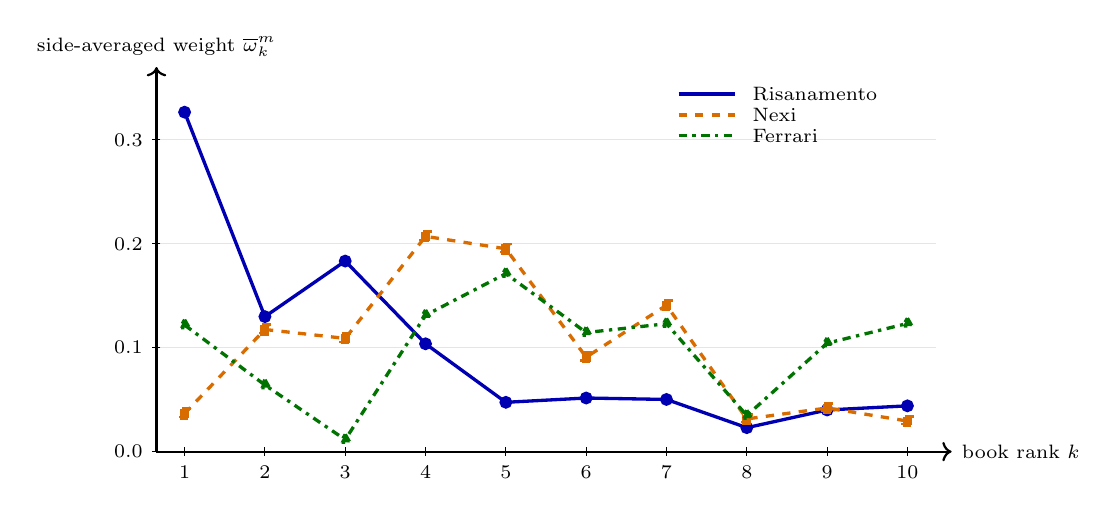
\begin{tikzpicture}[
        x=1.02cm,
        y=13.2cm,
        font=\scriptsize,
        axis/.style={->, thick},
        grid/.style={gray!20, thin},
        risanamento/.style={blue!70!black, very thick, mark=*, mark size=1.7pt},
        nexi/.style={orange!85!black, very thick, dashed, mark=square*, mark size=1.6pt},
        ferrari/.style={green!45!black, very thick, dash dot, mark=triangle*, mark size=1.9pt}
    ]
        \foreach \y in {0.1,0.2,0.3} {
            \draw[grid] (0.65,\y) -- (10.35,\y);
        }
        \draw[axis] (0.65,0) -- (10.55,0) node[right] {book rank $k$};
        \draw[axis] (0.65,0) -- (0.65,0.37) node[above, align=center]
            {side-averaged weight $\overline{\omega}^{m}_{k}$};

        \foreach \x in {1,...,10} {
            \draw (\x,0.004) -- (\x,-0.004) node[below] {\x};
        }
        \foreach \y/\lab in {0.0/$0.0$,0.1/$0.1$,0.2/$0.2$,0.3/$0.3$} {
            \draw (0.70,\y) -- (0.60,\y) node[left] {\lab};
        }

        \draw[risanamento]
            plot coordinates {
                (1,0.326590) (2,0.129904) (3,0.183346) (4,0.103747) (5,0.047449)
                (6,0.051590) (7,0.050207) (8,0.023040) (9,0.040075) (10,0.044052)
            };
        \draw[nexi]
            plot coordinates {
                (1,0.036660) (2,0.117508) (3,0.108946) (4,0.207104) (5,0.195161)
                (6,0.090903) (7,0.140818) (8,0.031470) (9,0.042001) (10,0.029429)
            };
        \draw[ferrari]
            plot coordinates {
                (1,0.121867) (2,0.064095) (3,0.011556) (4,0.131256) (5,0.171245)
                (6,0.114549) (7,0.123072) (8,0.034722) (9,0.104320) (10,0.123319)
            };

        \draw[risanamento] (7.15,0.344) -- (7.85,0.344);
        \node[anchor=west] at (7.95,0.344) {Risanamento};
        \draw[nexi] (7.15,0.324) -- (7.85,0.324);
        \node[anchor=west] at (7.95,0.324) {Nexi};
        \draw[ferrari] (7.15,0.304) -- (7.85,0.304);
        \node[anchor=west] at (7.95,0.304) {Ferrari};
    \end{tikzpicture}
    \caption{Full-sample empirical top-$10$ depth-kernel profiles at $H=10$ seconds. Each line is the arithmetic mean of
    the separately normalized bid and ask weights in \cref{eq:side_averaged_empirical_kernel}. The mean permits one curve
    per instrument on a common rank axis and is used only for visualization. Surveillance metrics use the underlying
    side-specific kernels.}
    \label{fig:empirical_top10_kernel_profiles}
\end{figure}
\FloatBarrier

To expose the two empirical inputs rather than only their normalized product,
\Cref{fig:empirical_topn_visibility_profiles,fig:empirical_topn_execution_risk_profiles} plot the side-specific
visibility and execution-risk profiles used in the calibration. The second plot reports
$\widehat p^{m,s}_{k}(H)$ directly; the
kernel uses its protection complement $\widehat\rho^{m,s}_{k}(H)=1-\widehat p^{m,s}_{k}(H)$. The plotted visibility component includes the numerical floor; the hit-frequency plot does not show the protection complement.

% Generated by scripts/generate_empirical_kernel_component_figures.py; do not edit manually.
% calibration root: outputs/depth_kernel_calibration/20260717_145624_rank_pooled_top10_h10
% source RISANAMENTO: outputs/depth_kernel_calibration/20260717_145624_rank_pooled_top10_h10/RISANAMENTO_top10_h10/empirical_depth_kernel.csv sha256=6ecb2071cf524f6090dff6596dc64248cbf59af2c55cf0d33e0649fcc52abe45
% source NEXI: outputs/depth_kernel_calibration/20260717_145624_rank_pooled_top10_h10/NEXI_top10_h10/empirical_depth_kernel.csv sha256=deaeb5a1c7a301d48c51347fbc4bdc2dc389281302aeb41192c20190920335f5
% source FERRARI: outputs/depth_kernel_calibration/20260717_145624_rank_pooled_top10_h10/FERRARI_top10_h10/empirical_depth_kernel.csv sha256=d5fdc562b059874471a511f2990341ceed08f434ddefb8b3cf31589979a67540

% data column: visibility_component
\begin{figure}[!ht]
\centering
\resizebox{\textwidth}{!}{%
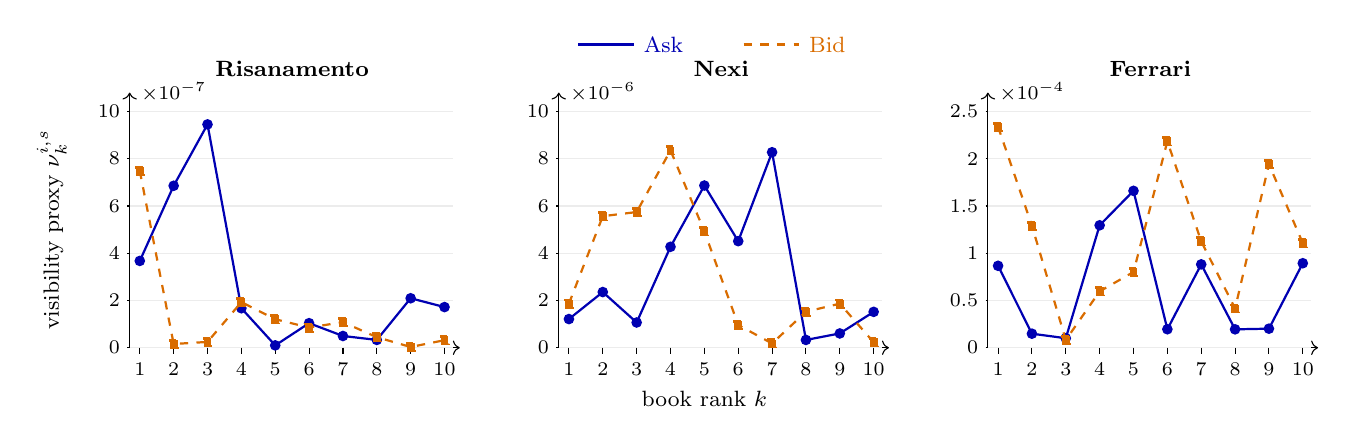
\begin{tikzpicture}
\begin{scope}[xshift=0.00cm]
\begin{scope}[x=0.43cm,y=0.30000000cm]
  \draw[->] (0.7,0) -- (10.45,0);
  \draw[->] (0.7,0) -- (0.7,10.8);
  \draw[gray!15] (0.7,0) -- (10.25,0);
  \draw (0.63,0) -- (0.7,0) node[left,font=\scriptsize] {0};
  \draw[gray!15] (0.7,2) -- (10.25,2);
  \draw (0.63,2) -- (0.7,2) node[left,font=\scriptsize] {2};
  \draw[gray!15] (0.7,4) -- (10.25,4);
  \draw (0.63,4) -- (0.7,4) node[left,font=\scriptsize] {4};
  \draw[gray!15] (0.7,6) -- (10.25,6);
  \draw (0.63,6) -- (0.7,6) node[left,font=\scriptsize] {6};
  \draw[gray!15] (0.7,8) -- (10.25,8);
  \draw (0.63,8) -- (0.7,8) node[left,font=\scriptsize] {8};
  \draw[gray!15] (0.7,10) -- (10.25,10);
  \draw (0.63,10) -- (0.7,10) node[left,font=\scriptsize] {10};
  \draw (1,0) -- (1,-0.025 * 10) node[below,font=\scriptsize] {1};
  \draw (2,0) -- (2,-0.025 * 10) node[below,font=\scriptsize] {2};
  \draw (3,0) -- (3,-0.025 * 10) node[below,font=\scriptsize] {3};
  \draw (4,0) -- (4,-0.025 * 10) node[below,font=\scriptsize] {4};
  \draw (5,0) -- (5,-0.025 * 10) node[below,font=\scriptsize] {5};
  \draw (6,0) -- (6,-0.025 * 10) node[below,font=\scriptsize] {6};
  \draw (7,0) -- (7,-0.025 * 10) node[below,font=\scriptsize] {7};
  \draw (8,0) -- (8,-0.025 * 10) node[below,font=\scriptsize] {8};
  \draw (9,0) -- (9,-0.025 * 10) node[below,font=\scriptsize] {9};
  \draw (10,0) -- (10,-0.025 * 10) node[below,font=\scriptsize] {10};
  \node[anchor=south west,font=\scriptsize] at (0.75,10) {$\times 10^{-7}$};
  \node[rotate=90,font=\footnotesize] at (-1.6,5) {visibility proxy $\nu_k^{i,s}$};
  \node[font=\footnotesize\bfseries] at (5.5,11.8) {Risanamento};
  \draw[blue!70!black, thick, mark=*, mark size=1.5pt] plot coordinates {(1,3.675229767983178) (2,6.855802152861837) (3,9.454395390358135) (4,1.6711452429542564) (5,0.09967103872544607) (6,1.03986078936913) (7,0.49722130939049286) (8,0.331027311346062) (9,2.094561089973038) (10,1.7209334991488594)};
  % RISANAMENTO ask visibility_component raw: 1:3.6752297679831775e-07, 2:6.855802152861836e-07, 3:9.4543953903581345e-07, 4:1.6711452429542563e-07, 5:9.9671038725446058e-09, 6:1.03986078936913e-07, 7:4.9722130939049281e-08, 8:3.31027311346062e-08, 9:2.0945610899730381e-07, 10:1.7209334991488592e-07
  \draw[orange!85!black, thick, dashed, mark=square*, mark size=1.4pt] plot coordinates {(1,7.4850054933810215) (2,0.15725764971410325) (3,0.24659322933232064) (4,1.930205433978854) (5,1.2069432758813796) (6,0.8540517059063696) (7,1.0836250920231838) (8,0.4466903180509029) (9,0.031098089940439774) (10,0.31967530278917544)};
  % RISANAMENTO bid visibility_component raw: 1:7.4850054933810209e-07, 2:1.5725764971410324e-08, 3:2.4659322933232062e-08, 4:1.9302054339788539e-07, 5:1.2069432758813797e-07, 6:8.5405170590636958e-08, 7:1.0836250920231838e-07, 8:4.4669031805090292e-08, 9:3.1098089940439771e-09, 10:3.1967530278917541e-08
\end{scope}
\end{scope}
\begin{scope}[xshift=5.45cm]
\begin{scope}[x=0.43cm,y=0.30000000cm]
  \draw[->] (0.7,0) -- (10.45,0);
  \draw[->] (0.7,0) -- (0.7,10.8);
  \draw[gray!15] (0.7,0) -- (10.25,0);
  \draw (0.63,0) -- (0.7,0) node[left,font=\scriptsize] {0};
  \draw[gray!15] (0.7,2) -- (10.25,2);
  \draw (0.63,2) -- (0.7,2) node[left,font=\scriptsize] {2};
  \draw[gray!15] (0.7,4) -- (10.25,4);
  \draw (0.63,4) -- (0.7,4) node[left,font=\scriptsize] {4};
  \draw[gray!15] (0.7,6) -- (10.25,6);
  \draw (0.63,6) -- (0.7,6) node[left,font=\scriptsize] {6};
  \draw[gray!15] (0.7,8) -- (10.25,8);
  \draw (0.63,8) -- (0.7,8) node[left,font=\scriptsize] {8};
  \draw[gray!15] (0.7,10) -- (10.25,10);
  \draw (0.63,10) -- (0.7,10) node[left,font=\scriptsize] {10};
  \draw (1,0) -- (1,-0.025 * 10) node[below,font=\scriptsize] {1};
  \draw (2,0) -- (2,-0.025 * 10) node[below,font=\scriptsize] {2};
  \draw (3,0) -- (3,-0.025 * 10) node[below,font=\scriptsize] {3};
  \draw (4,0) -- (4,-0.025 * 10) node[below,font=\scriptsize] {4};
  \draw (5,0) -- (5,-0.025 * 10) node[below,font=\scriptsize] {5};
  \draw (6,0) -- (6,-0.025 * 10) node[below,font=\scriptsize] {6};
  \draw (7,0) -- (7,-0.025 * 10) node[below,font=\scriptsize] {7};
  \draw (8,0) -- (8,-0.025 * 10) node[below,font=\scriptsize] {8};
  \draw (9,0) -- (9,-0.025 * 10) node[below,font=\scriptsize] {9};
  \draw (10,0) -- (10,-0.025 * 10) node[below,font=\scriptsize] {10};
  \node[anchor=south west,font=\scriptsize] at (0.75,10) {$\times 10^{-6}$};
  \node[font=\footnotesize\bfseries] at (5.5,11.8) {Nexi};
  \draw[blue!70!black, thick, mark=*, mark size=1.5pt] plot coordinates {(1,1.2138032154980023) (2,2.357195510456608) (3,1.0685006264223715) (4,4.273217243409157) (5,6.866026041374058) (6,4.512030446576142) (7,8.275878917434618) (8,0.32997233355025435) (9,0.6049414509297961) (10,1.5188249155682871)};
  % NEXI ask visibility_component raw: 1:1.2138032154980023e-06, 2:2.357195510456608e-06, 3:1.0685006264223715e-06, 4:4.2732172434091567e-06, 5:6.8660260413740573e-06, 6:4.5120304465761415e-06, 7:8.2758789174346172e-06, 8:3.2997233355025434e-07, 9:6.0494145092979615e-07, 10:1.5188249155682871e-06
  \draw[orange!85!black, thick, dashed, mark=square*, mark size=1.4pt] plot coordinates {(1,1.8674773855957816) (2,5.568884213770531) (3,5.7442838166896815) (4,8.353844420062963) (5,4.925771459538285) (6,0.9619962140487628) (7,0.1805094913160257) (8,1.5237267589959187) (9,1.8662709068477343) (10,0.2317283350241909)};
  % NEXI bid visibility_component raw: 1:1.8674773855957815e-06, 2:5.5688842137705302e-06, 3:5.7442838166896813e-06, 4:8.3538444200629627e-06, 5:4.9257714595382846e-06, 6:9.6199621404876272e-07, 7:1.8050949131602569e-07, 8:1.5237267589959187e-06, 9:1.8662709068477342e-06, 10:2.3172833502419091e-07
\end{scope}
\end{scope}
\begin{scope}[xshift=10.90cm]
\begin{scope}[x=0.43cm,y=1.20000000cm]
  \draw[->] (0.7,0) -- (10.45,0);
  \draw[->] (0.7,0) -- (0.7,2.7);
  \draw[gray!15] (0.7,0) -- (10.25,0);
  \draw (0.63,0) -- (0.7,0) node[left,font=\scriptsize] {0};
  \draw[gray!15] (0.7,0.5) -- (10.25,0.5);
  \draw (0.63,0.5) -- (0.7,0.5) node[left,font=\scriptsize] {0.5};
  \draw[gray!15] (0.7,1) -- (10.25,1);
  \draw (0.63,1) -- (0.7,1) node[left,font=\scriptsize] {1};
  \draw[gray!15] (0.7,1.5) -- (10.25,1.5);
  \draw (0.63,1.5) -- (0.7,1.5) node[left,font=\scriptsize] {1.5};
  \draw[gray!15] (0.7,2) -- (10.25,2);
  \draw (0.63,2) -- (0.7,2) node[left,font=\scriptsize] {2};
  \draw[gray!15] (0.7,2.5) -- (10.25,2.5);
  \draw (0.63,2.5) -- (0.7,2.5) node[left,font=\scriptsize] {2.5};
  \draw (1,0) -- (1,-0.025 * 2.5) node[below,font=\scriptsize] {1};
  \draw (2,0) -- (2,-0.025 * 2.5) node[below,font=\scriptsize] {2};
  \draw (3,0) -- (3,-0.025 * 2.5) node[below,font=\scriptsize] {3};
  \draw (4,0) -- (4,-0.025 * 2.5) node[below,font=\scriptsize] {4};
  \draw (5,0) -- (5,-0.025 * 2.5) node[below,font=\scriptsize] {5};
  \draw (6,0) -- (6,-0.025 * 2.5) node[below,font=\scriptsize] {6};
  \draw (7,0) -- (7,-0.025 * 2.5) node[below,font=\scriptsize] {7};
  \draw (8,0) -- (8,-0.025 * 2.5) node[below,font=\scriptsize] {8};
  \draw (9,0) -- (9,-0.025 * 2.5) node[below,font=\scriptsize] {9};
  \draw (10,0) -- (10,-0.025 * 2.5) node[below,font=\scriptsize] {10};
  \node[anchor=south west,font=\scriptsize] at (0.75,2.5) {$\times 10^{-4}$};
  \node[font=\footnotesize\bfseries] at (5.5,2.95) {Ferrari};
  \draw[blue!70!black, thick, mark=*, mark size=1.5pt] plot coordinates {(1,0.8669505020816368) (2,0.1485759198632677) (3,0.10059702674753057) (4,1.2956601892544413) (5,1.6603869526647457) (6,0.19557846353831482) (7,0.8821362998985953) (8,0.19476684019606572) (9,0.20169455861968041) (10,0.8943935007246941)};
  % FERRARI ask visibility_component raw: 1:8.6695050208163686e-05, 2:1.485759198632677e-05, 3:1.0059702674753058e-05, 4:0.00012956601892544412, 5:0.00016603869526647457, 6:1.9557846353831483e-05, 7:8.8213629989859532e-05, 8:1.9476684019606572e-05, 9:2.0169455861968043e-05, 10:8.9439350072469421e-05
  \draw[orange!85!black, thick, dashed, mark=square*, mark size=1.4pt] plot coordinates {(1,2.338679183565612) (2,1.291355118638466) (3,0.08201799287649617) (4,0.5966462138610819) (5,0.8015132512207448) (6,2.184977047983166) (7,1.1257505456756975) (8,0.41537003587522076) (9,1.9429973087449643) (10,1.1061392811485924)};
  % FERRARI bid visibility_component raw: 1:0.0002338679183565612, 2:0.00012913551186384661, 3:8.2017992876496163e-06, 4:5.9664621386108187e-05, 5:8.0151325122074484e-05, 6:0.00021849770479831661, 7:0.00011257505456756977, 8:4.1537003587522077e-05, 9:0.00019429973087449644, 10:0.00011061392811485925
\end{scope}
\end{scope}
\node[font=\footnotesize] at (7.6,-0.65) {book rank $k$};
\draw[blue!70!black,thick,mark=*,mark size=1.5pt] (6.0,3.85) -- (6.7,3.85) node[right,font=\footnotesize] {Ask};
\draw[orange!85!black,thick,dashed,mark=square*,mark size=1.4pt] (8.1,3.85) -- (8.8,3.85) node[right,font=\footnotesize] {Bid};
\end{tikzpicture}%
}
\caption{Side-specific empirical visibility proxy by book rank. Each panel shows the stored \texttt{visibility\_component} values from the full-sample top-$10$, $h=10$-second calibration. Separate axis multipliers preserve the instrument-specific price units; vertical magnitudes should not be compared across instruments.}
\label{fig:empirical_topn_visibility_profiles}
\end{figure}

% data column: hit_probability; protection_component = 1 - hit_probability
\begin{figure}[!ht]
\centering
\resizebox{\textwidth}{!}{%
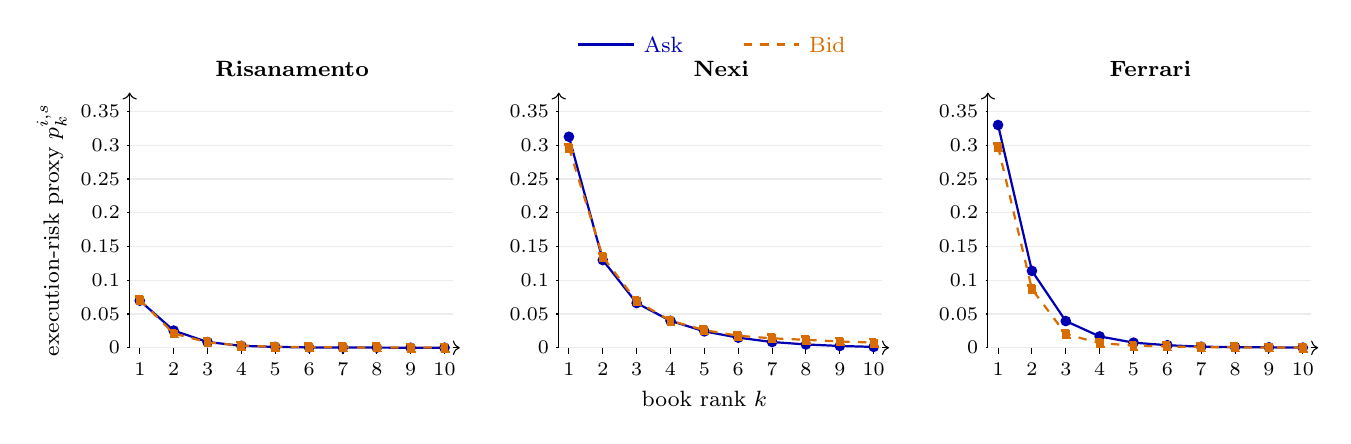
\begin{tikzpicture}
\begin{scope}[xshift=0.00cm]
\begin{scope}[x=0.43cm,y=8.57142857cm]
  \draw[->] (0.7,0) -- (10.45,0);
  \draw[->] (0.7,0) -- (0.7,0.378);
  \draw[gray!15] (0.7,0) -- (10.25,0);
  \draw (0.63,0) -- (0.7,0) node[left,font=\scriptsize] {0};
  \draw[gray!15] (0.7,0.05) -- (10.25,0.05);
  \draw (0.63,0.05) -- (0.7,0.05) node[left,font=\scriptsize] {0.05};
  \draw[gray!15] (0.7,0.1) -- (10.25,0.1);
  \draw (0.63,0.1) -- (0.7,0.1) node[left,font=\scriptsize] {0.1};
  \draw[gray!15] (0.7,0.15) -- (10.25,0.15);
  \draw (0.63,0.15) -- (0.7,0.15) node[left,font=\scriptsize] {0.15};
  \draw[gray!15] (0.7,0.2) -- (10.25,0.2);
  \draw (0.63,0.2) -- (0.7,0.2) node[left,font=\scriptsize] {0.2};
  \draw[gray!15] (0.7,0.25) -- (10.25,0.25);
  \draw (0.63,0.25) -- (0.7,0.25) node[left,font=\scriptsize] {0.25};
  \draw[gray!15] (0.7,0.3) -- (10.25,0.3);
  \draw (0.63,0.3) -- (0.7,0.3) node[left,font=\scriptsize] {0.3};
  \draw[gray!15] (0.7,0.35) -- (10.25,0.35);
  \draw (0.63,0.35) -- (0.7,0.35) node[left,font=\scriptsize] {0.35};
  \draw (1,0) -- (1,-0.025 * 0.35) node[below,font=\scriptsize] {1};
  \draw (2,0) -- (2,-0.025 * 0.35) node[below,font=\scriptsize] {2};
  \draw (3,0) -- (3,-0.025 * 0.35) node[below,font=\scriptsize] {3};
  \draw (4,0) -- (4,-0.025 * 0.35) node[below,font=\scriptsize] {4};
  \draw (5,0) -- (5,-0.025 * 0.35) node[below,font=\scriptsize] {5};
  \draw (6,0) -- (6,-0.025 * 0.35) node[below,font=\scriptsize] {6};
  \draw (7,0) -- (7,-0.025 * 0.35) node[below,font=\scriptsize] {7};
  \draw (8,0) -- (8,-0.025 * 0.35) node[below,font=\scriptsize] {8};
  \draw (9,0) -- (9,-0.025 * 0.35) node[below,font=\scriptsize] {9};
  \draw (10,0) -- (10,-0.025 * 0.35) node[below,font=\scriptsize] {10};
  \node[rotate=90,font=\footnotesize] at (-1.6,0.175) {execution-risk proxy $p_k^{i,s}$};
  \node[font=\footnotesize\bfseries] at (5.5,0.413) {Risanamento};
  \draw[blue!70!black, thick, mark=*, mark size=1.5pt] plot coordinates {(1,0.06972349940165018) (2,0.02545533573561784) (3,0.008478028770510227) (4,0.0028297304716921367) (5,0.0012412635498727) (6,0.0004097636793952453) (7,0.0002830315509421413) (8,0.00021971635327554557) (9,0.0) (10,0.0)};
  % RISANAMENTO ask hit_probability raw: 1:0.06972349940165018, 2:0.02545533573561784, 3:0.0084780287705102271, 4:0.0028297304716921367, 5:0.0012412635498726999, 6:0.0004097636793952453, 7:0.0002830315509421413, 8:0.00021971635327554557, 9:0, 10:0
  \draw[orange!85!black, thick, dashed, mark=square*, mark size=1.4pt] plot coordinates {(1,0.07096878130100093) (2,0.021101548570064722) (3,0.007994257645916313) (4,0.0031324298201674864) (5,0.0014088794806261372) (6,0.0008309423027754893) (7,0.0005630550368480321) (8,0.0003863103073313112) (9,0.00020106276030446647) (10,0.00018748873264827834)};
  % RISANAMENTO bid hit_probability raw: 1:0.070968781301000927, 2:0.021101548570064722, 3:0.0079942576459163129, 4:0.0031324298201674864, 5:0.0014088794806261372, 6:0.00083094230277548935, 7:0.00056305503684803214, 8:0.00038631030733131118, 9:0.00020106276030446647, 10:0.00018748873264827834
\end{scope}
\end{scope}
\begin{scope}[xshift=5.45cm]
\begin{scope}[x=0.43cm,y=8.57142857cm]
  \draw[->] (0.7,0) -- (10.45,0);
  \draw[->] (0.7,0) -- (0.7,0.378);
  \draw[gray!15] (0.7,0) -- (10.25,0);
  \draw (0.63,0) -- (0.7,0) node[left,font=\scriptsize] {0};
  \draw[gray!15] (0.7,0.05) -- (10.25,0.05);
  \draw (0.63,0.05) -- (0.7,0.05) node[left,font=\scriptsize] {0.05};
  \draw[gray!15] (0.7,0.1) -- (10.25,0.1);
  \draw (0.63,0.1) -- (0.7,0.1) node[left,font=\scriptsize] {0.1};
  \draw[gray!15] (0.7,0.15) -- (10.25,0.15);
  \draw (0.63,0.15) -- (0.7,0.15) node[left,font=\scriptsize] {0.15};
  \draw[gray!15] (0.7,0.2) -- (10.25,0.2);
  \draw (0.63,0.2) -- (0.7,0.2) node[left,font=\scriptsize] {0.2};
  \draw[gray!15] (0.7,0.25) -- (10.25,0.25);
  \draw (0.63,0.25) -- (0.7,0.25) node[left,font=\scriptsize] {0.25};
  \draw[gray!15] (0.7,0.3) -- (10.25,0.3);
  \draw (0.63,0.3) -- (0.7,0.3) node[left,font=\scriptsize] {0.3};
  \draw[gray!15] (0.7,0.35) -- (10.25,0.35);
  \draw (0.63,0.35) -- (0.7,0.35) node[left,font=\scriptsize] {0.35};
  \draw (1,0) -- (1,-0.025 * 0.35) node[below,font=\scriptsize] {1};
  \draw (2,0) -- (2,-0.025 * 0.35) node[below,font=\scriptsize] {2};
  \draw (3,0) -- (3,-0.025 * 0.35) node[below,font=\scriptsize] {3};
  \draw (4,0) -- (4,-0.025 * 0.35) node[below,font=\scriptsize] {4};
  \draw (5,0) -- (5,-0.025 * 0.35) node[below,font=\scriptsize] {5};
  \draw (6,0) -- (6,-0.025 * 0.35) node[below,font=\scriptsize] {6};
  \draw (7,0) -- (7,-0.025 * 0.35) node[below,font=\scriptsize] {7};
  \draw (8,0) -- (8,-0.025 * 0.35) node[below,font=\scriptsize] {8};
  \draw (9,0) -- (9,-0.025 * 0.35) node[below,font=\scriptsize] {9};
  \draw (10,0) -- (10,-0.025 * 0.35) node[below,font=\scriptsize] {10};
  \node[font=\footnotesize\bfseries] at (5.5,0.413) {Nexi};
  \draw[blue!70!black, thick, mark=*, mark size=1.5pt] plot coordinates {(1,0.31260453781443537) (2,0.12984782045855234) (3,0.06622282497020507) (4,0.03985550427610355) (5,0.024238887427669647) (6,0.014926477236300272) (7,0.008478372547005035) (8,0.004874179588448276) (9,0.002609710589260322) (10,0.0012329392037678621)};
  % NEXI ask hit_probability raw: 1:0.31260453781443537, 2:0.12984782045855234, 3:0.066222824970205069, 4:0.03985550427610355, 5:0.024238887427669647, 6:0.014926477236300272, 7:0.0084783725470050347, 8:0.0048741795884482764, 9:0.0026097105892603219, 10:0.0012329392037678621
  \draw[orange!85!black, thick, dashed, mark=square*, mark size=1.4pt] plot coordinates {(1,0.2962844238411685) (2,0.13459420361328928) (3,0.06890514548742396) (4,0.040104226602442915) (5,0.02609796394782051) (6,0.017697805652940525) (7,0.013941406635320423) (8,0.011730229384758923) (9,0.009260324871761146) (10,0.007653260445138618)};
  % NEXI bid hit_probability raw: 1:0.29628442384116849, 2:0.13459420361328928, 3:0.068905145487423963, 4:0.040104226602442915, 5:0.026097963947820511, 6:0.017697805652940525, 7:0.013941406635320423, 8:0.011730229384758923, 9:0.0092603248717611462, 10:0.0076532604451386181
\end{scope}
\end{scope}
\begin{scope}[xshift=10.90cm]
\begin{scope}[x=0.43cm,y=8.57142857cm]
  \draw[->] (0.7,0) -- (10.45,0);
  \draw[->] (0.7,0) -- (0.7,0.378);
  \draw[gray!15] (0.7,0) -- (10.25,0);
  \draw (0.63,0) -- (0.7,0) node[left,font=\scriptsize] {0};
  \draw[gray!15] (0.7,0.05) -- (10.25,0.05);
  \draw (0.63,0.05) -- (0.7,0.05) node[left,font=\scriptsize] {0.05};
  \draw[gray!15] (0.7,0.1) -- (10.25,0.1);
  \draw (0.63,0.1) -- (0.7,0.1) node[left,font=\scriptsize] {0.1};
  \draw[gray!15] (0.7,0.15) -- (10.25,0.15);
  \draw (0.63,0.15) -- (0.7,0.15) node[left,font=\scriptsize] {0.15};
  \draw[gray!15] (0.7,0.2) -- (10.25,0.2);
  \draw (0.63,0.2) -- (0.7,0.2) node[left,font=\scriptsize] {0.2};
  \draw[gray!15] (0.7,0.25) -- (10.25,0.25);
  \draw (0.63,0.25) -- (0.7,0.25) node[left,font=\scriptsize] {0.25};
  \draw[gray!15] (0.7,0.3) -- (10.25,0.3);
  \draw (0.63,0.3) -- (0.7,0.3) node[left,font=\scriptsize] {0.3};
  \draw[gray!15] (0.7,0.35) -- (10.25,0.35);
  \draw (0.63,0.35) -- (0.7,0.35) node[left,font=\scriptsize] {0.35};
  \draw (1,0) -- (1,-0.025 * 0.35) node[below,font=\scriptsize] {1};
  \draw (2,0) -- (2,-0.025 * 0.35) node[below,font=\scriptsize] {2};
  \draw (3,0) -- (3,-0.025 * 0.35) node[below,font=\scriptsize] {3};
  \draw (4,0) -- (4,-0.025 * 0.35) node[below,font=\scriptsize] {4};
  \draw (5,0) -- (5,-0.025 * 0.35) node[below,font=\scriptsize] {5};
  \draw (6,0) -- (6,-0.025 * 0.35) node[below,font=\scriptsize] {6};
  \draw (7,0) -- (7,-0.025 * 0.35) node[below,font=\scriptsize] {7};
  \draw (8,0) -- (8,-0.025 * 0.35) node[below,font=\scriptsize] {8};
  \draw (9,0) -- (9,-0.025 * 0.35) node[below,font=\scriptsize] {9};
  \draw (10,0) -- (10,-0.025 * 0.35) node[below,font=\scriptsize] {10};
  \node[font=\footnotesize\bfseries] at (5.5,0.413) {Ferrari};
  \draw[blue!70!black, thick, mark=*, mark size=1.5pt] plot coordinates {(1,0.3299702364891511) (2,0.1138451000944385) (3,0.039512737809105136) (4,0.016772763406691257) (5,0.007550976354941552) (6,0.0037028504060889473) (7,0.0015255640954857832) (8,0.0008800569546293279) (9,0.0005811708933011752) (10,0.00019095892515032825)};
  % FERRARI ask hit_probability raw: 1:0.32997023648915108, 2:0.1138451000944385, 3:0.039512737809105136, 4:0.016772763406691257, 5:0.0075509763549415519, 6:0.0037028504060889473, 7:0.0015255640954857832, 8:0.00088005695462932789, 9:0.00058117089330117521, 10:0.00019095892515032825
  \draw[orange!85!black, thick, dashed, mark=square*, mark size=1.4pt] plot coordinates {(1,0.29774219794269774) (2,0.08683487342980731) (3,0.0201937386748806) (4,0.006785226513236277) (5,0.003250439515049369) (6,0.0018722238366059196) (7,0.0007970509116269802) (8,0.0005189144310103264) (9,0.0003238052933862769) (10,0.00017228173668293312)};
  % FERRARI bid hit_probability raw: 1:0.29774219794269774, 2:0.086834873429807308, 3:0.020193738674880599, 4:0.0067852265132362774, 5:0.003250439515049369, 6:0.0018722238366059196, 7:0.00079705091162698017, 8:0.00051891443101032637, 9:0.0003238052933862769, 10:0.00017228173668293312
\end{scope}
\end{scope}
\node[font=\footnotesize] at (7.6,-0.65) {book rank $k$};
\draw[blue!70!black,thick,mark=*,mark size=1.5pt] (6.0,3.85) -- (6.7,3.85) node[right,font=\footnotesize] {Ask};
\draw[orange!85!black,thick,dashed,mark=square*,mark size=1.4pt] (8.1,3.85) -- (8.8,3.85) node[right,font=\footnotesize] {Bid};
\end{tikzpicture}%
}
\caption{Side-specific empirical execution-risk proxy by book rank. The plotted quantity is the stored $h$-second reach probability $p_k^{i,s}$ (\texttt{hit\_probability}) from the full-sample top-$10$, $h=10$-second calibration. The empirical kernel uses its protection complement $\rho_k^{i,s}=1-p_k^{i,s}$.}
\label{fig:empirical_topn_execution_risk_profiles}
\end{figure}

\FloatBarrier

We can now summarize each side of the participant's complete profile. The weighted liquidity averages the participant's share of market depth at each rank using the calibrated kernel:
\begin{equation}
    L^{i,s}_{n}(t)
    =
    \sum_{k=1}^{n}
    \omega^{s}_{k}(t)\,\widetilde V^{i,s}_{k}(t).
    \label{eq:weighted_topn_liquidity}
\end{equation}
To compare sides without making the result depend on the overall size of that weighted footprint, we divide their difference by their sum. This defines the \textit{Multilevel Distance-Weighted Imbalance}:
\begin{equation}
    \operatorname{DWI}^{i}_{n}(t)
    =\begin{cases}
    \dfrac{
        L^{i,a}_{n}(t)-L^{i,b}_{n}(t)
    }{
        L^{i,a}_{n}(t)+L^{i,b}_{n}(t)
    },
    & L^{i,a}_{n}(t)+L^{i,b}_{n}(t)>0,\\
    \text{undefined},
    & L^{i,a}_{n}(t)+L^{i,b}_{n}(t)=0.
    \end{cases}
    \label{eq:multilevel_dwi}
\end{equation}
Positive DWI denotes an ask-heavy weighted profile; negative DWI denotes a bid-heavy one. Dividing by total weighted liquidity makes the statistic describe the balance between sides rather than the absolute size of the footprint, within a fixed instrument and kernel. Values near $+1$ and $-1$ correspond to almost entirely ask-side and bid-side profiles. A value near zero instead means that positive weighted liquidity is balanced between sides.

The absence of liquidity is different from balance. The ratio in \cref{eq:multilevel_dwi} is undefined when both weighted sides are absent. The reconstructed series uses a separate recording convention for the one-time transition when a previously observed top-$n$ profile disappears: it assigns zero to that explicit operational state. This recorded zero marks disappearance, not a balanced positive profile; it does not make the ratio mathematically defined. Other undefined ratios remain missing.

Setting $n=1$ gives the best-level measure; larger $n$ also includes liquidity behind the touch. DWI describes profile shape. Neither its level nor its change selects candidate orders or determines the strict gate. The paths in \cref{fig:topn_imbalance_dynamics} illustrate this distinction rather than define an empirical classification rule.

\begin{figure}[htbp]
    \centering
    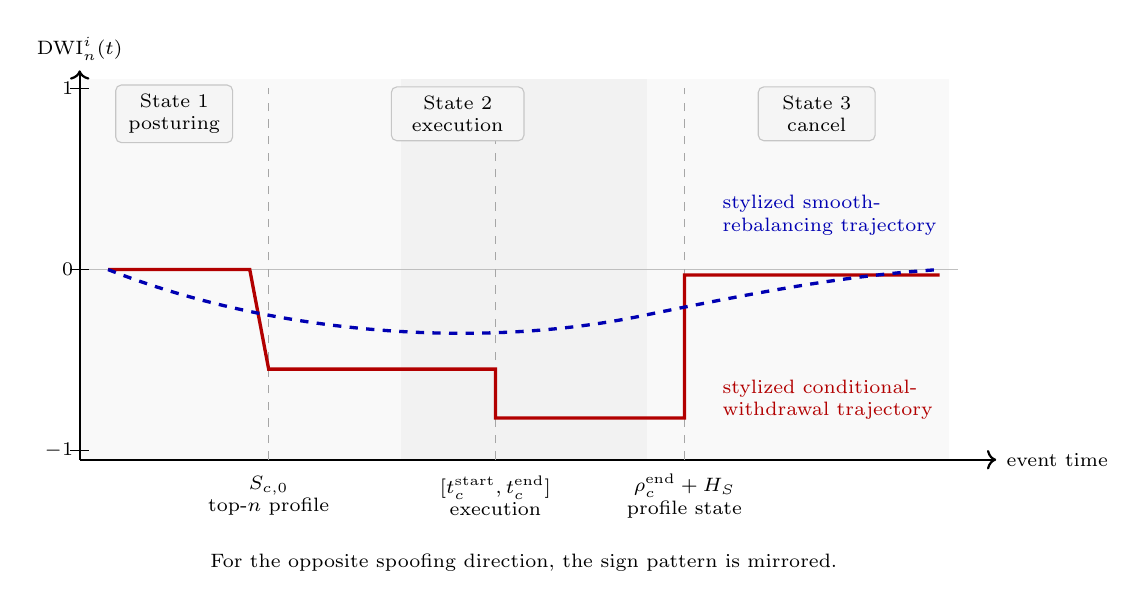
\begin{tikzpicture}[
        x=2.4cm,
        y=2.3cm,
        font=\scriptsize,
        axis/.style={->, thick},
        spoof/.style={very thick, red!70!black},
        maker/.style={very thick, dashed, blue!70!black},
        event/.style={gray!70, dashed},
        state/.style={fill=gray!8, draw=gray!45, rounded corners=2pt, align=center}
    ]
        \fill[gray!5] (0,-1.05) rectangle (1.7,1.05);
        \fill[gray!10] (1.7,-1.05) rectangle (3.0,1.05);
        \fill[gray!5] (3.0,-1.05) rectangle (4.6,1.05);

        \draw[axis] (0,-1.05) -- (0,1.1) node[above] {$\operatorname{DWI}_{n}^{i}(t)$};
        \draw[axis] (0,-1.05) -- (4.85,-1.05) node[right] {event time};
        \draw[gray!50] (-0.05,0) -- (4.65,0);

        \foreach \y/\lab in {-1/$-1$,0/$0$,1/$1$} {
            \draw (-0.05,\y) -- (0.05,\y) node[left=0.08cm] {\lab};
        }

        \draw[event] (1.0,-1.05) -- (1.0,1.0);
        \draw[event] (2.2,-1.05) -- (2.2,1.0);
        \draw[event] (3.2,-1.05) -- (3.2,1.0);

        \node[state, text width=1.25cm] at (0.5,0.86) {State 1\\posturing};
        \node[state, text width=1.45cm] at (2.0,0.86) {State 2\\execution};
        \node[state, text width=1.25cm] at (3.9,0.86) {State 3\\cancel};

        \node[align=center] at (1.0,-1.25) {$S_{c,0}$\\top-$n$ profile};
        \node[align=center] at (2.2,-1.25) {$[t_c^{\mathrm{start}},t_c^{\mathrm{end}}]$\\execution};
        \node[align=center] at (3.2,-1.25) {$\rho_c^{\mathrm{end}}+H_S$\\profile state};

        \draw[spoof] (0.15,0) -- (0.9,0)
            -- (1.0,-0.55) -- (2.2,-0.55)
            -- (2.2,-0.82) -- (3.2,-0.82)
            -- (3.2,-0.03) -- (4.55,-0.03);

        \draw[maker] (0.15,0) .. controls (1.0,-0.35) and (2.1,-0.45) .. (3.0,-0.25)
            .. controls (3.7,-0.10) and (4.1,-0.03) .. (4.55,0);

        \node[red!70!black, align=left, anchor=west] at (3.35,-0.72) {stylized conditional-\\withdrawal trajectory};
        \node[blue!70!black, align=left, anchor=west] at (3.35,0.30) {stylized smooth-\\rebalancing trajectory};
        \node[align=center] at (2.35,-1.62) {For the opposite spoofing direction, the sign pattern is mirrored.};
    \end{tikzpicture}
    \caption{Stylized execution-time behavior of the multilevel distance-weighted imbalance. The conditional-withdrawal
    trajectory shows a large top-$n$ imbalance returning rapidly toward zero after the opposite-side execution. The smooth
    trajectory illustrates gradual rebalancing. Neither trajectory is an empirical classification rule.}
    \label{fig:topn_imbalance_dynamics}
\end{figure}
\FloatBarrier

\subsubsection{Conditional Withdrawal Reconstruction}
\label{subsec:multilevel_conditionality}

An imbalanced profile alone does not distinguish the two economic benchmarks: a market maker may also quote asymmetrically. We therefore ask what changes after the participant executes on the opposite side. We first compare the complete profile before and after execution, then follow the recent orders separately. This preserves the distinction between a change in book shape and cancellation of specific liquidity.

Let $c$ denote an execution by participant $i$, formed from the related messages defined in \cref{sec:data}.
Those messages share a trading partition, participant, order, role, and side, and satisfy the stated gap rule.
Passive executions share a resting price; aggressive executions use traded prices and quantities and may span several
price levels. Write $Q_c$ for total executed quantity, $s_c\in\{b,a\}$ for execution side, and $\bar{s}_c$ for the opposite side.

There are two notions of sequence to preserve. Trading times locate the execution economically, while source positions determine which messages have already been applied to the book. Sequence-clock times measure order age and locate the later profile. For execution $c$, let $t_c^{\mathrm{start}}$ and $t_c^{\mathrm{end}}$ be the first and last trade times, $r_c^{\mathrm{first}}$ and $r_c^{\mathrm{last}}$ their source positions, and $\rho_c^{\mathrm{start}}$ and $\rho_c^{\mathrm{end}}$ their sequence-clock times.

Book states are saved after messages are applied in source order. We use $t_c^{-}$ and $t_c^{+}$ as labels for selected book states, not as alternative execution timestamps. The pre-execution state $t_c^{-}$ is the last retained participant state strictly before the first execution message. Its saved market price need not be the global book price immediately before that message.

For the later comparison, we set $\rho_c^{\mathrm{target}}=\rho_c^{\mathrm{end}}+H_S$, with $H_S=10$ seconds. The state $t_c^{+}$ is the last retained state at or before that target whose source index is no smaller than the final execution message's index. The profile-change measures below---SCI, $C^{i,s}_{c,n}$, and MSCI---are undefined if either required state is unavailable.

For the candidate orders, we impose an additional recency requirement. This prevents liquidity that has been resting
for a long time from entering the candidate set simply because it happens to be present at execution.
If $\tau_o$ is the order's first observed posting time on the sequence clock, its age must lie within $\Theta>0$:
\begin{equation}
    0 \leq \rho_c^{\mathrm{start}}-\tau_o \leq \Theta .
    \label{eq:deceptive_age_window}
\end{equation}
We use $\Theta=90$ seconds as an exploratory default. The candidate set $\mathcal{P}^{i,\bar{s}_c}_{c,n,\Theta}$ consists
of participant $i$'s orders that are active immediately before the first execution message, lie on the opposite side
within the first $n$ ranks, and satisfy \cref{eq:deceptive_age_window}. We fix the set at that point, recording each
order's visible quantity, rank, weighted relative depth, and first-observed time. The total candidate quantity is
\begin{equation}
    Q^{i,\bar{s}_c}_{c,n}
    =
    \sum_{o\in\mathcal{P}^{i,\bar{s}_c}_{c,n,\Theta}} q_o(t_c^{-}).
    \label{eq:age_conditioned_candidate_quantity}
\end{equation}
This restriction applies to the orders followed for withdrawal, to the withdrawal-based review score, and to the final
selection. It does not remove older orders from the complete profile. Keeping the complete profile allows us to see
whether the participant changes liquidity on both sides, even when only a recent subset supplies the candidate sequence.

Our first comparison asks how much the imbalance changes between these two states, irrespective of direction. The \textit{Spoofing Conditionality Index} is the absolute change in DWI:
\begin{equation}
    \operatorname{SCI}^{i}_{c,n}
    =
    \left|
        \operatorname{DWI}^{i}_{n}(t_c^{-})
        -
        \operatorname{DWI}^{i}_{n}(t_c^{+})
    \right|.
    \label{eq:topn_sci}
\end{equation}
SCI measures the magnitude of the imbalance change, but not which side loses liquidity. A profile can become less bid-heavy because bid liquidity decreases or because ask liquidity increases. We therefore supplement SCI with a separate measure of decrease on each side:
\begin{equation}
    C^{i,s}_{c,n}
    =\begin{cases}
    \dfrac{
        \left[
            L^{i,s}_{n}(t_c^{-})-L^{i,s}_{n}(t_c^{+})
        \right]_{+}
    }{
        L^{i,s}_{n}(t_c^{-})
    },
    & L^{i,s}_{n}(t_c^{-})>0,\\
    0,
    & L^{i,s}_{n}(t_c^{-})=0.
    \end{cases}
    \qquad s\in\{b,a\}.
    \label{eq:side_collapse}
\end{equation}
Here $[x]_{+}=\max\{x,0\}$ keeps only decreases in weighted liquidity. The ratio expresses that decrease as a fraction of the side's pre-execution footprint. Thus $C^{i,s}_{c,n}=1$ means that the entire weighted footprint on side $s$ disappeared, while $C^{i,s}_{c,n}=0$ means that it did not decrease or was initially absent. A large $C^{i,\bar{s}_c}_{c,n}$ describes a decrease opposite to the execution. A two-sided quote refresh may instead generate decreases on both sides.

The second comparison asks which side loses weighted liquidity. A decrease opposite to the execution contributes positively to an asymmetric-collapse description; a decrease on the execution side offsets it. We combine that difference with half the absolute imbalance change to define the signed multilevel profile conditionality measure (MSCI):
\begin{equation}
    \operatorname{MSCI}^{i}_{c,n}
    =\frac{1}{2}\operatorname{SCI}^{i}_{c,n}
     +C^{i,\bar{s}_c}_{c,n}
     -C^{i,s_c}_{c,n}.
    \label{eq:signed_msci}
\end{equation}
DWI lies in $[-1,1]$, so $\operatorname{SCI}/2$ and each collapse term lie in $[0,1]$. MSCI consequently lies in $[-1,2]$ without clipping. A positive value means that the imbalance change and opposite-side decrease outweigh the execution-side decrease. A negative value means that the execution-side decrease dominates; zero is the neutral contrast.

The positive part in $C$ excludes growth from each decrease term, but MSCI itself remains signed. It is a comparison of the complete, market-relative top-$n$ profile, not a measure of attributed cancellation. In particular, growth on one side can change DWI and produce positive MSCI without cancellation. Fills, rank migration, changes in market depth, and later cancellations can also change the profile.

We retain SCI and both side-specific decreases so that the reason for an MSCI value remains visible. MSCI is a secondary diagnostic in participant-level feature summaries. It is neither a probability nor proof that liquidity was withdrawn, and it does not enter the four-condition selection or the reported result tables. Its range applies only when both required states are observed; otherwise it is missing.

Because the complete profile includes older orders, long-lived balanced liquidity can dilute its measured change. This is not an error in the profile comparison: it reflects a different question. MSCI describes the participant's overall displayed position, whereas the measures below ask what happened to the recent candidate orders.

\subsubsection{Canonical Matched Withdrawal}
\label{subsec:canonical_matched_withdrawal}

We now move from the complete profile to the recent candidate orders. Their withdrawal creates an attribution problem: one cancellation may follow several eligible executions by the participant. Counting the cancellation after each execution would overstate the quantity withdrawn. We therefore retain all eligible connections but assign each physical cancellation to one execution.

Let $j$ denote a physical cancellation message and $o(j)$ its order lifecycle. The order index $o$ used in the candidate set is distinct from the cancellation index $j$. A cancellation is eligible for assignment only when the cancelled order belongs to the execution's fixed candidate set, the participant is the same, and the execution is on the opposite side.

Eligibility also requires both source-order precedence and a short economic delay. The cancellation must follow the final execution message in source order. It must satisfy $0\leq \rho_j-t_c^{\mathrm{end}}<\Delta\tau_W$, with cancellation time $\rho_j$ on the sequence clock and $\Delta\tau_W=2$ seconds. This mixed-clock delay is evaluated in integer nanoseconds under the common-origin assumption. Let $\mathcal E(j)$ be the executions satisfying these conditions. We select one by
\begin{equation}
    a(j)=\underset{c\in\mathcal E(j)}{\arg\min}\,
    \left(-r_c^{\mathrm{last}},\;r_c^{\mathrm{first}},\;\operatorname{id}_c\right),
    \label{eq:canonical_cancel_assignment}
\end{equation}
The tuple is compared lexicographically, one entry at a time. The negative final source position makes the latest eligible execution take priority. Any remaining tie is resolved by the earlier first source position and then a stable execution identifier. Thus assignment follows message order, not the shortest delay between the two clocks. A shortest-economic-delay rule is examined separately as an alternative. As explained in \cref{sec:data}, checking the delay requires the common-timebase assumption.

The set $\mathcal{C}_{c,n}^{i}=\{j:a(j)=c\}$ collects the eligible top-$n$ cancellations assigned to execution $c$.
We identify a physical cancellation by trading partition, source index, and order identifier. All eligible links are
retained for inspection, but only the selected link contributes to withdrawal totals.

Assignment alone does not determine how much quantity to count. An order may increase in size between execution and cancellation, but that added quantity was not in the candidate profile. For an assigned cancellation $j\in\mathcal{C}_{c,n}^{i}$, let $q^{\mathrm{pre}}_{c,o(j)}=q_{o(j)}(t_c^{-})$ be the order's visible quantity immediately before execution and $q^{\mathrm{cancel}}_j$ its quantity immediately before cancellation. We count the smaller of the two:
\begin{equation}
    \bar q_{c,j}
    =
    \min\!\left\{q^{\mathrm{pre}}_{c,o(j)},q^{\mathrm{cancel}}_j\right\}.
    \label{eq:attributed_cancel_quantity}
\end{equation}
This cap excludes later quantity increases from attributed withdrawal. We retain the uncapped quantity at cancellation for inspection. Summing the capped quantities gives total assigned withdrawal. Dividing by executed quantity then compares the two scales:
\begin{equation}
    U^{i}_{c,n}=\sum_{j\in\mathcal{C}_{c,n}^{i}}\bar q_{c,j},
    \qquad
    R^{i}_{c,n}=\frac{U^{i}_{c,n}}{Q_c},
    \label{eq:assigned_withdrawal}
\end{equation}
where $Q_c>0$ is the execution quantity by construction. Using the age-conditioned candidate quantity
$Q^{i,\bar{s}_c}_{c,n}$ from \cref{eq:age_conditioned_candidate_quantity}, we report the fraction of that profile removed as
\begin{equation}
    A^{i}_{c,n}
    =\begin{cases}
    \dfrac{U^{i}_{c,n}}{Q^{i,\bar{s}_c}_{c,n}},
    & Q^{i,\bar{s}_c}_{c,n}>0,\\
    \text{undefined},
    & Q^{i,\bar{s}_c}_{c,n}=0.
    \end{cases}
    \label{eq:assigned_withdrawal_share}
\end{equation}
The ratios use different denominators because they answer different questions. $R^{i}_{c,n}$ asks how large withdrawal is relative to the execution. It can exceed one. $A^{i}_{c,n}$ asks how much of the candidate quantity is removed. The quantity cap and unique physical-cancellation assignment keep this share in $[0,1]$ whenever its denominator is positive. An absent candidate set makes the share undefined, rather than zero.

Two executions may be followed by the same withdrawn quantity but at different delays. To give earlier withdrawal
greater weight when prioritizing review, we define
\begin{equation}
    \widetilde U^{i}_{c,n}
    =
    \sum_{j\in\mathcal{C}_{c,n}^{i}}
    \bar q_{c,j}\exp\!\left(-\frac{\rho_j-t_c^{\mathrm{end}}}{\tau_w}\right),
    \qquad \tau_w=10\ \text{seconds}.
    \label{eq:delay_weighted_withdrawal}
\end{equation}
Within the $2$-second assignment window, an earlier cancellation receives a larger exponential weight. The scale $\tau_w$ determines how much the review score discounts delay; it is not an estimated causal response rate. We now combine candidate size relative to execution, weighted withdrawal relative to execution, and the share of candidates removed. The resulting \textit{Withdrawal Multilevel Spoofing Conditionality Index} is
\begin{equation}
    \operatorname{WMSCI}^{i}_{c,n}
    =
    \begin{cases}
    \displaystyle
    \log\!\left(1+\frac{Q^{i,\bar{s}_c}_{c,n}}{Q_c}\right)
    \log\!\left(1+\frac{\widetilde U^{i}_{c,n}}{Q_c}\right)
    A^{i}_{c,n},
    & Q^{i,\bar{s}_c}_{c,n}>0\ \text{and}\ \widetilde U^{i}_{c,n}>0,\\[5pt]
    0,
    & Q^{i,\bar{s}_c}_{c,n}=0\ \text{or}\ \widetilde U^{i}_{c,n}=0.
    \end{cases}
    \label{eq:wmsci}
\end{equation}
The first logarithm measures how large the candidate posture is relative to the execution. The second measures the quantity withdrawn on the same execution-relative scale, after discounting delay. Multiplying by $A^{i}_{c,n}$ distinguishes cancellation of a small part of the posture from more complete removal. The logarithms compress large quantity ratios rather than impose a maximum score.

WMSCI is zero when there is no candidate quantity or no delay-weighted assigned withdrawal. Otherwise it is non-negative and has no fixed upper bound. A zero score does not imply that the complete resting profile stayed unchanged: orders outside the candidate set may still have changed.

It is important to interpret this score as gross withdrawal. The assigned quantity $U^{i}_{c,n}$ counts capped cancellation from fixed candidate orders without subtracting new or replacement submissions. The participant can therefore cancel much of that layer while maintaining the same total displayed liquidity.

The score's components are related algebraically, so they should not be interpreted as independent dimensions of behavior. To make that dependence explicit, we suppress indices for a single execution with positive candidate and assigned quantities. Write $P=Q^{i,\bar{s}_c}_{c,n}$, $Q=Q_c$, $U=U^{i}_{c,n}$, and $\alpha=\widetilde U^{i}_{c,n}/U$. Here $A$ and $R$ abbreviate the removal share and withdrawal-to-execution ratio already defined, and $\alpha$ is the mean delay discount. These abbreviations also apply in the component tables.

The definitions give $A=U/P$ and $R=U/Q$, hence $R=A(P/Q)$. Substituting these identities gives $\operatorname{WMSCI}=A\log(1+R/A)\log(1+\alpha R)$. Thus the score combines transformations of the same quantities. Scaling all quantities together leaves the ratios unchanged. Changing the denominator or assigning a cancellation to a different execution can change the score.

We use decreasing WMSCI to order executions for human review. It is not a probability or a proportional scale of suspiciousness. The episode selection in \cref{subsec:event_reconstruction} instead uses quantity and price conditions, with no WMSCI threshold. At participant--partition level, counts and withdrawal rates describe activity; execution scores are not converted into a participant ranking.

\subsubsection{Price-Response Diagnostics}
\label{subsec:price_response_diagnostics}

The next question is whether the observed withdrawal accompanies the price pattern that motivates the hypothesized strategy. The participant would benefit from a favorable movement while the displayed orders are present, followed by reversion after withdrawal. We measure these two stages separately from WMSCI. Otherwise, large cancellation could be mistaken for evidence that the expected price response occurred.

We use two price proxies. Let $b(t)$ and $a(t)$ be the best bid and ask, with total displayed market quantities $D^b_1(t)$ and $D^a_1(t)$. These are the rank-1 depths already defined above, not participant or individual-order quantities. The midprice is $M_{\mathrm{mid}}(t)=[a(t)+b(t)]/2$. The queue microprice is $M_{\mathrm{micro}}(t)=[a(t)D^b_1(t)+b(t)D^a_1(t)]/[D^b_1(t)+D^a_1(t)]$ \cite{Stoikov02122018}; it weights the quotes by the opposite queues. The corresponding diagnostic is missing unless both quotes and positive top-level depth are available. Write $M(t)$ for either proxy; the calibration quantity $M^m(t)$ above is specifically the midprice of instrument $m$.

A favorable-movement measure needs a placement benchmark. Let $r_{c,0}$ be the largest first-observed source position among the eligible candidate postings. The placement benchmark $S_{c,0}$ is the exact saved book state immediately after that selected message, and $M(S_{c,0})$ is its price. Thus the benchmark is indexed by source position, not by a potentially non-unique timestamp. It marks completion of the fixed candidate layer, even when several postings share a timestamp. The selected source position must be strictly before the first execution message; otherwise, or if the saved state is unavailable, the diagnostic is missing. We then encode execution direction as
\begin{equation}
    h_c=
    \begin{cases}
        +1, & \text{if the execution is a sell execution,}\\
        -1, & \text{if the execution is a buy execution.}
    \end{cases}
    \label{eq:price_response_direction}
\end{equation}
A sell benefits from an upward price move, while a buy benefits from a downward one. With this sign convention, both produce a positive favorable price movement (FPM). We compare the price at completion of the candidate layer with the saved price in the selected pre-execution participant state:
\begin{equation}
    \operatorname{FPM}^{i}_{c}
    =
    h_c\left[M(t_c^{-})-M(S_{c,0})\right],
    \label{eq:favorable_price_move}
\end{equation}
Reversion (REV) asks whether the price later moves against that favorable direction. Its clock therefore starts at each assigned cancellation, not at execution. Let $M_j^{\mathrm{saved}}$ be the price in the last retained participant state strictly before cancellation $j$ in source order, and let $H_R=2$ seconds be the observation horizon. This saved benchmark need not coincide with the market state immediately before that message. Write $M_j^H$ for the price in the retained horizon state selected at or before $\rho_j+H_R$, provided the message sequence covers the target. The set $\mathcal{C}_{c,n}^{i,\mathrm{obs}}$ retains assigned cancellations with both price observations and a finite positive weight $w_{c,j}>0$. We average their signed changes with quantity-and-delay weights:
\begin{equation}
    \operatorname{REV}^{i}_{c}
    =
    \frac{
        \sum_{j\in\mathcal{C}_{c,n}^{i,\mathrm{obs}}}
        w_{c,j}h_c\left[M_j^{\mathrm{saved}}-M_j^H\right]
    }{
        \sum_{j\in\mathcal{C}_{c,n}^{i,\mathrm{obs}}} w_{c,j}
    },
    \qquad
    w_{c,j}=\bar q_{c,j}\exp\!\left(-\frac{\rho_j-t_c^{\mathrm{end}}}{\tau_w}\right),
    \label{eq:price_reversion}
\end{equation}
with $\tau_w=10$ seconds in the reported run. The statistic is undefined when no assigned cancellation
contributes a finite positive weight with both required price observations.

The recorded price path around cancellation can contain several contributions. We distinguish a gap between the retained benchmark and the physical state immediately before cancellation, the immediate quote change at cancellation, and the later path. For an assigned cancellation $j$, use the same reversion sign $-h_c$ as in \cref{eq:price_reversion}. It is $+1$ for a bid (buy) execution and $-1$ for an ask (sell) execution. The saved benchmark $M_j^{\mathrm{saved}}$ and observed horizon price $M_j^H$ are those used in REV. Denote the exact market prices immediately before and after the cancellation message by $M_j^{-}$ and $M_j^{+}$. In ticks, the decomposition is the accounting identity
\begin{equation}
\frac{-h_c(M_j^H-M_j^{\mathrm{saved}})}{\mathrm{tick}}
=\frac{-h_c(M_j^{-}-M_j^{\mathrm{saved}})}{\mathrm{tick}}
+\frac{-h_c(M_j^{+}-M_j^{-})}{\mathrm{tick}}
+\frac{-h_c(M_j^H-M_j^{+})}{\mathrm{tick}}.
\label{eq:observed_rev_decomposition}
\end{equation}
The three terms on the right are, respectively, the baseline gap, immediate recorded jump, and subsequent observed movement. This decomposition helps locate a price change in the recorded path. It does not remove the participant's remaining liquidity or construct the price that would have prevailed without cancellation. REV retains the quantity-and-delay weights and observation requirements defined above, and the strict gate does not use this decomposition. Missing decomposition components remain missing, not zero.

A positive $\operatorname{FPM}^{i}_{c}$ means that the price moved favorably between candidate-layer completion and execution. A positive $\operatorname{REV}^{i}_{c}$ means that the observed proxy moved against that favorable direction after the assigned cancellation or cancellations. A third comparison uses the quantity-weighted execution price $\bar p_c$ rather than a later book price. We define execution advantage (ADV) relative to the placement benchmark by
\begin{equation}
    \operatorname{ADV}^{i}_{c}
    =
    h_c\left[\bar p_c-M(S_{c,0})\right].
    \label{eq:execution_advantage}
\end{equation}
The execution advantage is positive when a sell executes above the benchmark or a buy executes below it.

The event records contain both midprice and queue-microprice diagnostics; the summary tables and episode gate use midprice. The formulas above are in price units. Reported FPM, REV, and ADV are divided by the instrument's tick size to express them in ticks; the decomposition already includes that conversion. Keeping FPM, REV, and ADV separate from withdrawal makes the distinction explicit: one set of variables describes order cancellation, while the other describes the associated price path. An execution can exhibit substantial withdrawal without favorable movement or subsequent reversion. The joint episode selection below asks when those features occur together.

\subsubsection{Event Reconstruction}
\label{subsec:event_reconstruction}

We can now assemble the measurements into episodes. The reconstruction must first distinguish actual order changes from changes in rank. When the best quote moves, an unchanged order can occupy a different rank without being amended or cancelled. Order-level messages preserve that distinction; aggregate snapshots alone cannot identify withdrawal by the participant.

For each execution $c$, formed from compatible messages in source order, the reconstructed book immediately before its first message determines each active order's side and rank. We fix the recent opposite-side candidates $\mathcal{P}^{i,\bar{s}_c}_{c,n,\Theta}$ from that pre-message book.

The complete-profile comparison instead uses the retained participant states selected above. The earlier state supplies the weighted quantities $L^{i,b}_{n}(t_c^{-})$ and $L^{i,a}_{n}(t_c^{-})$, and $\operatorname{DWI}^{i}_{n}(t_c^{-})$. We follow the complete profile to $\rho_c^{\mathrm{end}}+H_S$ and select $t_c^{+}$ by the earlier state rule. Its comparison with $t_c^{-}$ yields SCI, the two side-specific decreases, and MSCI. These selected records must not be confused with exact global book states adjacent to the execution message.

For the fixed candidates, we identify eligible cancellations, assign each once using \cref{eq:canonical_cancel_assignment}, and cap its quantity using \cref{eq:attributed_cancel_quantity}. These operations give the execution's withdrawal quantity, execution-relative ratio, candidate share removed, and WMSCI. Its price comparisons start from the saved state after the last candidate posting in source order and follow the path through execution and the post-cancellation horizon.

Several executions can occur while the same candidate orders remain displayed. Counting them as separate episodes would fragment a continuing posture. We connect executions sharing at least one candidate-order lifecycle within the same participant, execution side, trading partition, and recorded event date. Each connected component is a \emph{candidate-posture episode} $e$. The connection can be indirect: executions linked through another member belong to the same component. We retain each member's passive or aggressive role and count each physical cancellation once. Participant--day recurrence then counts distinct episodes, with member executions and original messages retained for inspection.

Selection is applied to the episode as a whole. Let $\mathcal{E}_e$ be its member executions and $Q_e=\sum_{c\in\mathcal{E}_e}Q_c$ their total executed quantity. The episode's withdrawal $U_e$ sums attributed quantity over unique physical cancellations. We average $\operatorname{FPM}_e$ with execution-quantity weights and $\operatorname{REV}_e$ with the quantity-and-delay weights of unique withdrawals. FPM is missing if any member lacks its required favorable-movement observation. REV is missing if any assigned cancellation lacks its required reversion observation.

The strict \textit{spoofing-compatible sequence} gate asks whether all four features are present together:
\begin{enumerate}
    \item At least one eligible opposite-side cancellation is canonically assigned within $2$ seconds of a member execution.
    \item Unique attributed withdrawal exceeds total executed quantity: $U_e>Q_e>0$.
    \item Observed midprice favorable movement is strictly positive: $\operatorname{FPM}_e>0$.
    \item Observed midprice reversion after cancellation is strictly positive: $\operatorname{REV}_e>0$.
\end{enumerate}
This conjunction selects complete observed sequences, not executions above a WMSCI threshold. A member can have zero assigned withdrawal because a shared cancellation was assigned to another member. Missing or right-censored prices fail selection, but must be distinguished from observed nonpositive prices.

The reported specification uses a $10$-second structural window, $2$-second rapid-attribution and cancel-anchored reversion
windows, and a $90$-second candidate-order age limit. We estimate the empirical top-$10$ kernel separately for each
instrument. Withdrawal and price-response components remain separate rather than being reduced to a scalar composite score.

\section{Results}
\label{sec:results}

We ask whether execution-conditioned withdrawal also exhibits the price pattern that motivates the hypothesized spoofing strategy. We first establish which executions have recent opposite-side liquidity and subsequent assigned withdrawal. We then compare the withdrawal score with changes in the complete resting profile and with the observed price path. Timing and recurrence provide complementary evidence, before we examine the episodes that jointly satisfy the quantity and price conditions and the sensitivity of these results to operational choices.

The populations narrow along two related paths, summarized in \cref{fig:results_selection_map}. Positive WMSCI selects executions with assigned withdrawal. The strict selection instead evaluates shared candidate-posture episodes; it is not a further cutoff on WMSCI. This distinction matters because a selected episode can contain executions with zero assigned withdrawal.

\begin{figure}[!htbp]
    \centering
    \begin{singlespace}
    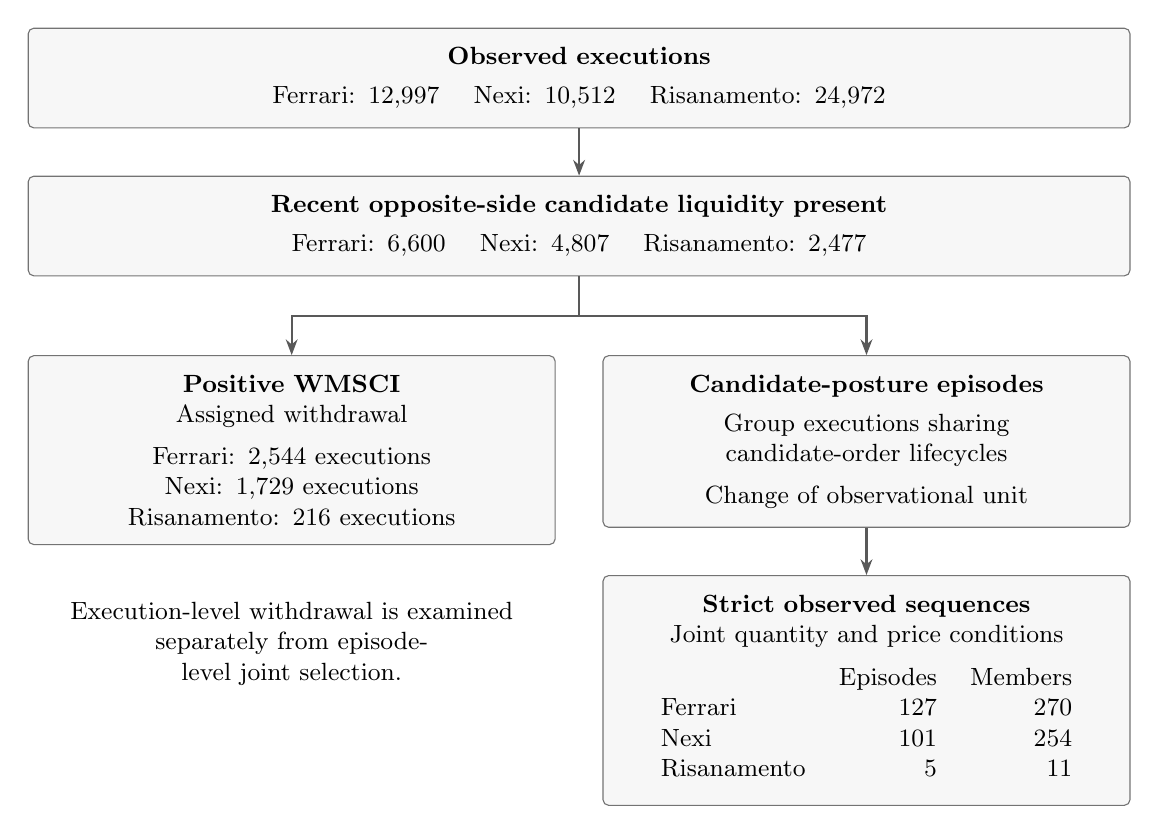
\begin{tikzpicture}[
        font=\small,
        roadmapbox/.style={draw=black!55, rounded corners=2pt, align=center,
            inner sep=7pt, text width=6.2cm, fill=black!3},
        roadmaparrow/.style={-{Stealth[length=2mm]}, thick, draw=black!65}
    ]
        \node[roadmapbox, text width=13.5cm] (all)
            {\textbf{Observed executions}\\[3pt]
             Ferrari: 12,997 \quad Nexi: 10,512 \quad Risanamento: 24,972};
        \node[roadmapbox, text width=13.5cm, below=6mm of all] (candidate)
            {\textbf{Recent opposite-side candidate liquidity present}\\[3pt]
             Ferrari: 6,600 \quad Nexi: 4,807 \quad Risanamento: 2,477};
        \node[roadmapbox, anchor=north] (positive)
            at ([xshift=-3.65cm,yshift=-10mm]candidate.south)
            {\textbf{Positive WMSCI}\\
             Assigned withdrawal\\[4pt]
             Ferrari: 2,544 executions\\
             Nexi: 1,729 executions\\
             Risanamento: 216 executions};
        \node[roadmapbox, anchor=north] (episode)
            at ([xshift=3.65cm,yshift=-10mm]candidate.south)
            {\textbf{Candidate-posture episodes}\\[3pt]
             Group executions sharing\\
             candidate-order lifecycles\\[4pt]
             Change of observational unit};
        \node[roadmapbox, below=6mm of episode] (strict)
            {\textbf{Strict observed sequences}\\
             Joint quantity and price conditions\\[5pt]
             \begin{tabular}{@{}lrr@{}}
                 & Episodes & Members\\
                 Ferrari & 127 & 270\\
                 Nexi & 101 & 254\\
                 Risanamento & 5 & 11
             \end{tabular}};
        \coordinate (branch) at ([yshift=-5mm]candidate.south);
        \draw[roadmaparrow] (all.south) -- (candidate.north);
        \draw[thick, draw=black!65] (candidate.south) -- (branch);
        \draw[roadmaparrow] (branch) -| (positive.north);
        \draw[roadmaparrow] (branch) -| (episode.north);
        \draw[roadmaparrow] (episode.south) -- (strict.north);
        \node[align=center, text width=6.2cm, below=6mm of positive]
            {Execution-level withdrawal is examined\\
             separately from episode-level joint selection.};
    \end{tikzpicture}
    \end{singlespace}
    \caption{Observation and selection paths. Positive WMSCI requires assigned withdrawal from recent opposite-side candidates. The separate episode gate requires rapid assigned cancellation, unique withdrawal exceeding total executed quantity, positive favorable midprice movement, and positive cancellation-anchored reversion. Members are executions belonging to selected episodes, including some with zero WMSCI. Arrows denote filtering or grouping, not causal effects; box sizes are not proportional to counts.}
    \label{fig:results_selection_map}
\end{figure}

\subsection{Observation and attribution}
\label{subsec:observation_attribution_results}
\label{subsec:cross_instrument_results}
\label{subsec:risanamento_results}
\label{subsec:nexi_results}
\label{subsec:ferrari_results}

The observation population narrows at two successive steps: recent opposite-side liquidity must first be present, and some of it must then be assigned to withdrawal. The samples contain 12,997 Ferrari, 10,512 Nexi, and 24,972 Risanamento executions. Candidate liquidity is present before 6,600, 4,807, and 2,477 executions, respectively. Positive WMSCI is observed for 2,544, 1,729, and 216 executions. \Cref{tab:withdrawal-population} reports these nested execution populations.

Complete-profile comparisons have different observation requirements. MSCI is unavailable for 333 Ferrari, 621 Nexi, and 4,610 Risanamento executions. We keep these missing observations distinct from zero MSCI. Neither the execution counts nor positive-score counts are episode counts. The Candidates column counts executions with candidate liquidity, not individual candidate orders.

\input{generated/withdrawal_characterization_v1/population.tex}

The available identity also differs across executions. Original client codes identify 4,344 Ferrari, 5,902 Nexi, and 20,722 Risanamento executions; the remaining 8,653, 4,610, and 4,250 use firm fallback. Because a firm may pool several clients, a firm-level sequence cannot automatically be interpreted as one client's behavior. All subsequent comparisons retain this distinction.

The results use the source-order cancellation assignment and the candidate-layer completion benchmark defined in the model. Assignment gives priority to the latest eligible execution message. FPM and ADV use the saved state after the last candidate posting in source order. Comparisons between execution and cancellation times retain the common-timebase assumption in \cref{sec:data}.

Temporal coverage limits the interpretation of repetition. Ferrari and Nexi each contain executions on one day; Risanamento contains them on 129 days. Of Risanamento's 130 raw-input partitions, one has no execution. Reconstructed windows reach the end of every retained partition, avoiding observed partition-end censoring of withdrawal. This check does not establish feed completeness, uninterrupted sessions, or independence between executions.
\FloatBarrier

\subsection{Continuous withdrawal characterization}
\label{subsec:continuous_withdrawal_results}

Most executions have zero withdrawal score. Among those with positive WMSCI, the score largely orders gross withdrawal in the same way as the simpler withdrawal-to-execution ratio $R$. Spearman correlations are 0.944027 in Ferrari, 0.952082 in Nexi, and 0.978366 in Risanamento. This relation is consistent with the algebraic coupling of the score's components. In the component table, Spearman reports the association of each component with WMSCI. The positive-score distributions in \cref{fig:withdrawal_wmsci_ecdf} describe the remaining variation, with zero-score mass reported separately.

The ordering also depends on which eligible execution receives a shared cancellation. The allocation comparison in \cref{subsec:withdrawal_sensitivity_results} changes execution-level ranks while leaving strict episode selection unchanged. This dependence matters for the order of human review, even though the aggregate episode counts agree.

WMSCI nevertheless changes some of the ordering because it also weights the share of candidate liquidity removed. Its top 1\%, 5\%, and 10\% tails overlap the corresponding $R$ tails by 16/26, 94/128, and 199/255 in Ferrari; 9/18, 59/87, and 133/173 in Nexi; and 3/3, 11/11, and 22/22 in Risanamento. These fractions count executions common to both tails relative to the tail size. In tail tables, $k$ is the selected number of executions, not a book rank; the two uses are confined to their respective contexts. The score thus largely follows $R$, with a removal-share adjustment that changes the tails in Ferrari and Nexi. The comparison does not establish that this adjustment gives a better economic ranking.

\begin{figure}[!htbp]
    \centering
    \includegraphics[width=0.92\textwidth]{generated/withdrawal_characterization_v1/wmsci_ecdf.pdf}
    \caption{Empirical cumulative distributions conditional on positive WMSCI, plotted against log(1+WMSCI). The legend reports positive counts and the separate full-population zero mass. WMSCI describes gross, capped, uniquely attributed cancellation relative to the execution under the stated allocation.}
    \label{fig:withdrawal_wmsci_ecdf}
\end{figure}
\input{generated/withdrawal_characterization_v1/components.tex}
\input{generated/withdrawal_characterization_v1/tail_overlap.tex}

Large attributed cancellation need not produce a large change in the complete resting profile. The joint distribution in \cref{fig:withdrawal_msci_wmsci_joint} does not reproduce WMSCI ordering along MSCI. The two statistics measure different objects: WMSCI follows assigned cancellation from recent candidates, while MSCI describes the participant's complete market-relative top-$10$ profile. Missing MSCI is excluded from this joint plot, not replaced by zero.

Reviews of individual order lifecycles make the distinction concrete. In a maximum-MSCI Ferrari observation, candidate orders were filled rather than cancelled. In a high-WMSCI Risanamento observation, assigned withdrawal is $U=150{,}000$ against execution quantity $Q=157$, yet the participant displays 150,000 units in the top-$10$ book both before and after because liquidity is replenished. These cases illustrate how gross cancellation, net displayed quantity, and weighted profile shape can differ. They do not measure how often the distinction occurs.

\begin{figure}[!htbp]
    \centering
    \includegraphics[width=0.88\textwidth]{generated/withdrawal_characterization_v1/msci_wmsci_joint.pdf}
    \caption{Joint distribution of positive WMSCI and finite MSCI on common axes and a common logarithmic color scale. Color represents execution counts per common hexagonal bin. The vertical coordinate is log(1+WMSCI). Zeros and missing MSCI are retained in population accounting rather than displayed as joint-score observations.}
    \label{fig:withdrawal_msci_wmsci_joint}
\end{figure}
\FloatBarrier

\subsection{Behavioral versus price-path evidence}
\label{subsec:behavior_price_results}

Does greater withdrawal accompany a more favorable price path? The positive-WMSCI population does not show a consistent increase in favorable movement as the score rises. Pooling passive and aggressive executions and both attribution levels within each instrument, the Spearman association with FPM is $-0.004543$ in Ferrari, $-0.011687$ in Nexi, and $-0.131444$ in Risanamento. This pooled summary does not establish that execution roles or client and firm attribution units are interchangeable.

The price summaries and distributions below show the comparisons separately for each diagnostic. These descriptive associations do not rule out a price effect; they show that WMSCI does not uniformly order favorable movement in the observed samples.

\input{generated/withdrawal_characterization_v1/price_associations.tex}
\input{generated/withdrawal_characterization_v1/joint_price.tex}
\begin{figure}[!htbp]
    \centering
    \includegraphics[width=\textwidth]{generated/withdrawal_characterization_v1/price_diagnostics.pdf}
    \caption{Observed price distributions across WMSCI groups. Rows show favorable midprice movement (FPM), cancel-anchored midprice reversion (REV), and execution advantage relative to candidate-layer completion (ADV), all in ticks; columns show Ferrari, Nexi, and Risanamento. Candidate-present executions are divided into the separate zero-W group and five instrument-specific positive-score quintiles. Violins show kernel density estimates with Scott's bandwidth over the full observed range, normalized to equal maximum width; black horizontal lines mark sample medians, not confidence intervals. Each panel has its own vertical scale, and its title reports the total observed count. Missing prices are omitted, including unobserved REV at zero W. Sparse or constant samples are shown without a density estimate. ADV is a benchmark difference, not realized profit.}
    \label{fig:withdrawal_price_diagnostics}
    \label{fig:withdrawal_price_fpm}
    \label{fig:withdrawal_price_rev}
    \label{fig:withdrawal_price_adv}
\end{figure}

The highest scores also do not uniformly accompany the two favorable price signs together. At the pooled positive-WMSCI top-5\% cutoff, Ferrari has 128 executions with both FPM and native REV observed, of which 15 have both measures positive. Nexi has 86 observed pairs, of which 14 have both positive; Risanamento has 11, of which none does. One selected Nexi event lacks a complete pair and is missing, not unfavorable.

ADV answers another question: how the execution price compares with the candidate-placement benchmark. It uses the execution's volume-weighted average price and the same benchmark as FPM. Subtracting FPM from ADV leaves the signed execution-price difference from the saved midprice in the selected pre-execution state. This execution edge is not realized profit.

\FloatBarrier

The decomposition asks whether positive reversion is confined to the immediate quote change recorded at cancellation. Among strict episodes, the later observed path remains positive for 127/127 Ferrari, 100/101 Nexi, and 4/5 Risanamento episodes. This is a description of episodes already selected for positive native REV, not independent validation of their price pattern.

The decomposition uses a $10^{-10}$-tick threshold to distinguish positive later movement from numerically tiny values. The strict gate itself retains literal positivity. Excluding the immediate recorded jump also does not exclude the participant's full remaining book or provide a causal counterfactual.

\input{generated/withdrawal_characterization_v1/rev_decomposition.tex}
\FloatBarrier

\subsection{Timing and recurrence of execution-conditioned withdrawal}
\label{subsec:timing_recurrence_results}

The price comparisons do not tell us whether cancellation is concentrated at execution time. To examine timing, we compare windows centered on observed execution with windows shifted by $-60$, $-30$, $+30$, and $+60$ seconds. This is a separate analysis of dynamically eligible liquidity, not the fixed candidate population used by WMSCI.

The timing contrast first compares cancellation intensity in passive-only or aggressive-only own-execution windows with a reference period containing no attributed own-execution window. The reference means no observed window under the attribution rule, not that the participant did no economic trading. We repeat that contrast after shifting the execution schedule.

Within each instrument--identity--role stratum, we determine eligibility anew at every offset. We retain groups supported at all offsets and hold their zero-offset exposure weights fixed. Actual exposure is recomputed at each offset and may differ. The outcome is physical cancellations per posture-second: cancellation count divided by the time over which eligible liquidity is exposed. The zero-offset estimate is thus a within-sample timing comparison, not the full observed-population estimate or a validation of score ranking.
\input{generated/withdrawal_characterization_v1/timing.tex}

Cancellation is concentrated at the zero-offset window in Ferrari and Nexi, in both original-client and firm-fallback strata. Risanamento does not show a unique zero-offset peak. Its firm-fallback comparison is also sparse, with only two firm-fallback identities. The timing summaries retain the exposure and participant support needed to interpret each comparison, with finer strata in the supplementary material. The contrast localizes activity within these samples; it does not supply an otherwise matched causal counterfactual.

\FloatBarrier

The upper score tail also contains repeated activity by a small set of participants. Its 128 Ferrari, 87 Nexi, and 11 Risanamento executions occupy 124, 80, and 11 episodes, respectively, and involve 10, 7, and 1 actors. Executions and episodes therefore provide different counts of repetition, and tail observations are not independent replications.

Ferrari and Nexi each cover one trading day, so their repetition cannot establish performance on an unseen day. Risanamento's 11 tail episodes belong to one firm on different days. Because that identity is a firm rather than an original client, the pattern does not establish persistence by one client.
\input{generated/withdrawal_characterization_v1/recurrence.tex}
\FloatBarrier

\subsection{Strict observed-sequence subset}
\label{subsec:strict_sequence_subset_results}

Applying the four conditions jointly selects a small observed spoofing-compatible subset: 127 Ferrari, 101 Nexi, and 5 Risanamento episodes. Those episodes contain 270, 254, and 11 executions, respectively. Of their member executions, 89, 89, and 6 have zero assigned withdrawal. This is possible because selection is applied to the combined episode, while a shared cancellation is assigned to only one member.

The selected episodes also differ in attribution and role composition. Original-client counts are 8, 12, and 3; firm-fallback counts are 119, 89, and 2. Mixed-role episodes number 22, 15, and 1; these are labeled Mixed anchors in the table. Such episodes contain both passive and aggressive executions and cannot be added independently across role categories.
\input{generated/withdrawal_characterization_v1/strict.tex}

High withdrawal scores seldom coincide with strict episode membership. In the top 5\% WMSCI tails, 16 of 128 Ferrari executions, 14 of 87 Nexi executions, and 0 of 11 Risanamento executions belong to a selected episode. Most high-score executions therefore lie outside the joint sequence subset, as shown in \cref{fig:strict_score_space}.

This contrast follows from the different questions asked by the score and the gate. The score describes withdrawal, whereas the gate also requires the quantity condition and strictly positive ($>0$) price diagnostics. Strict status and its selected price observations have no independent label or validation. The subset is not a confirmed class or a severity ranking.

\begin{figure}[!htbp]
    \centering
    \includegraphics[width=0.88\textwidth]{generated/withdrawal_characterization_v1/strict_score_space.pdf}
    \caption{All finite-MSCI executions in grey, with orange circles marking execution members of episodes selected by the four-condition gate. Axes are MSCI and log(1+WMSCI), including zero W. Episode membership is not equivalent to an execution independently passing every strict condition; repeated shared postures are not independent observations.}
    \label{fig:strict_score_space}
\end{figure}
\input{generated/withdrawal_characterization_v1/strict_tail.tex}
\FloatBarrier

\subsection{Withdrawal-sensitivity characterization}
\label{subsec:withdrawal_sensitivity_results}

The withdrawal ranking depends on which eligible execution receives a cancellation. Comparing the source-order assignment with the alternative based on economic delay gives top-tail overlaps of 92/128 in Ferrari, 73/87 in Nexi, and 10/11 in Risanamento. The receiving execution changes for 567, 489, and 22 retained physical cancellations, respectively; score rank correlations are 0.490119, 0.538640, and 0.743033. The strict episode flags remain unchanged, at 127, 101, and 5 episodes. Thus these allocations change execution-level ordering even when episode selection agrees. They compare distinct attribution policies, not numerical perturbations of one policy.

Changing delay weighting and changing eligibility have different consequences. Narrower decay choices mostly preserve the ordering. By contrast, shortening the rapid-withdrawal window to 1 second and then 0.5 seconds removes eligible connections. Positive-WMSCI Risanamento executions attributed to original clients fall from 49 to 10 to 4. These are original-client counts, not pooled Risanamento counts.

Requiring $Q_c\geq 10$ also changes the eligible execution population. The retained top-tail counts are 13/128 in Ferrari, 82/87 in Nexi, and 11/11 in Risanamento. The native gate is not recomputed after episode members are removed. Consequently, these comparisons describe a changed population rather than a newly defined episode screen. Appendix Tables~\ref{tab:withdrawal-score-sensitivity} and~\ref{tab:withdrawal-gate-sensitivity} give the full grids. We do not report sensitivity to top-$n$, candidate age, the execution-grouping gap, or a larger structural window.
\FloatBarrier

\section{Discussion and Conclusion}
\label{sec:discussion_conclusion}

Following individual orders makes it possible to connect display, execution, and withdrawal without inferring their motive. The continuous score measures gross cancellation from a fixed set of recent orders. Its denominators show how large that set and the withdrawal are relative to executed quantity. Because replacement orders are not subtracted, even substantial attributed withdrawal can leave the participant's displayed liquidity unchanged.

The empirical ordering is largely explained by the simpler withdrawal-to-execution ratio. This is consistent with the score combining related transformations of the same quantities. The additional removal-share and timing weights can change the ranking, but the evidence does not establish a uniformly better economic ordering. Assignment priority also changes execution-level ranking even when strict episode selection agrees. The contribution is therefore an inspectable description of withdrawal, with its components and denominators available, rather than a validated severity scale.

Neither the complete profile nor the price path can be inferred from gross cancellation alone. New orders may keep the profile stable or increase it while recent candidates disappear. Likewise, larger withdrawal scores do not consistently accompany more favorable price diagnostics. The reversion decomposition locates movement in the immediate recorded quote change and the later path. It does not determine the price that would have prevailed without the participant's withdrawal.

The timing and recurrence results depend on what the sample can identify. A firm may combine several clients, and executions sharing displayed orders are not independent observations. Ferrari and Nexi each cover one execution-bearing day, so these samples cannot evaluate recurrence on a held-out day. The separate timing analysis uses dynamically eligible liquidity rather than the fixed candidates behind WMSCI. Its heterogeneous results describe when cancellation occurs; they do not validate the score or establish a universal withdrawal mechanism.

The strict subset provides a complementary episode-level summary. It retains sequences where withdrawal quantity and the two price signs meet their conditions together. A member execution need not satisfy every condition on its own, because the gate evaluates the shared episode. Moreover, favorable movement and reversion are selection criteria, not independent confirmation afterward. Without adjudicated labels, the subset cannot estimate classification error or manipulation prevalence.

Stronger conclusions require a different evaluation design. Independently evidenced legitimate liquidity providers would provide a relevant comparison population. Samples with enough days would permit chronological validation. An own-book counterfactual would require order-level depth information and an explicit reconstruction excluding the participant's liquidity. Alternative placement benchmarks and broader eligibility or grouping choices likewise require new calculations, rather than reinterpretation of the retained links. Sensitivity to book depth, candidate age, the execution-grouping gap, and a larger structural window remains untested.

The current analysis also assumes a common origin for trade and sequence clocks and estimates the empirical kernel on the full sample. Subject to those limits, its results support descriptive review of observable sequences. They do not establish manipulative intent or causal price impact.

% We propose two agent-specific metrics based on the
% microprice and the volume-distance correlation. 
% \paragraph{Agent-Specific Microprice ($m_i$)} The traditional microprice is widely 
% recognized in high-frequency trading as a robust estimator of the expected future midprice \cite{Stoikov02122018}, uniquely synthesizing both
% the price and volume dimensions of the limit order book. By isolating this calculation to a single participant's resting 
% orders, we can formulate an an agent-specific microprice ($m_i$) to quantify its personal vision of the future price::

% \begin{equation}
%     m_i = \frac{a_iV^b_i + b_i V^a_i}{V^b_i + V^a_i} = \frac{a_i + b_i}{2} + \frac{a_i-b_i}{2} \frac{V_i^b-V_i^a}{V_i^b+V_i^a} = \text{midprice} + \frac{\text{spread}}{2} \times \text{imbalance}
% \end{equation}
% Where $a_i$ and $b_i$ represent the agent's ask and bid prices, and $V^a_i$ and $V^b_i$ represent their respective 
% volumes. Legitimate market makers, constrained by inventory risk, typically maintain symmetric quotes ($V^b_i \approx V^a_i$) 
% to capture the spread, resulting in an $m_i$ that closely tracks the fundamental midprice. Conversely, a spoofer
% deliberately engineers an extreme unbalanced environment to manipulate the heuristics of victim algorithms. 
% Consequently, a spoofer's $m_i$ will drastically diverge from the true midprice.

% \paragraph{Correlation Between Posting Distance ($\delta$) and Volume} The second metric mathematically formalizes the 
% spoofer's optimization dilemma by measuring the correlation between an agent's order volume and their posting distance 
% ($\delta$) from the best bid or ask. Empirical models confirm that posting distance is a critical determinant of price 
% impact, and its omission renders LOB detection models mathematically inadequate.Because market makers seek execution to 
% earn the bid-ask spread, their inventory management necessitates posting their largest order volumes at or adjacent to 
% the top of the book ($\delta \approx 0$). Spoofers, conversely, optimize a strictly directional expected cost function: 
% they must maximize the psychological and algorithmic impact of their non-bona fide volume while minimizing the risk of 
% inadvertent execution. This is achieved by placing a small, bona fide order at a minimal distance ($\delta \approx 0$) 
% to guarantee execution, and a massive, non-bona fide order at a significantly larger distance deeper within the opposite 
% side of the LOB ($\delta \gg 0$) to act as a structural buffer against aggressive market orders. Thus, observing a strong 
% correlation between massive volume and a large $\delta$ on one side of the book—paired with small volume and a minimal 
% $\delta$ on the execution side—serves as and additional microstructural signature of a manipulative strategy.


\FloatBarrier
\appendix
\section{Diagnostic Scope and Reproducibility}
\label{sec:withdrawal_diagnostics}

\subsection{Population, identity, and price coverage}
The supplementary aggregates keep passive and aggressive executions separate, and distinguish original-client from firm-fallback attribution. Pooling provides a descriptive summary, not evidence that the strata are interchangeable. Counts of executions, episodes, and execution membership in episodes use different denominators. A zero withdrawal score can coexist with selected episode membership or a change in the complete resting profile. Missing profile and price observations remain missing.

In the supplementary tables, Events and Members count executions, Actors count participant identities at the reported attribution level, and strict component denotes a strict selected episode. The Favourable + REV column counts executions with both FPM and native REV observed and positive. Component-table A, Q, and R denote the candidate removal share, executed quantity, and withdrawal-to-execution ratio, respectively.

Compact table and plot labels use W for WMSCI and M for MSCI; M in those labels is not the price proxy $M(t)$.

Price coverage is reported separately for each diagnostic and stratum. Within each instrument, positive scores define five quintiles; zero-score executions form a separate group, not the first quintile. The violins summarize observed distributions and mark sample medians, not confidence intervals. Sparse or constant samples are displayed without a density estimate. The association summaries do not establish calibrated population uncertainty, given repeated postures, unequal day coverage, and selection on observed outcomes.

\subsection{Tails, recurrence, and opportunity}
Tail comparisons require a consistent selection rule. The main exact-$k$ tails use deterministic ordering within the stated positive-score population. Supplementary tie-inclusive tails also retain observations tied at the boundary, which can increase the denominator. Their overlaps cannot be reported as if the two rules selected identical populations. Recurrence and opportunity summaries separately retain execution counts, distinct postures, actors, and available actor-day coverage. Firm-level repetition need not be repetition by one client.

The timing comparison includes only groups supported at every offset and holds their zero-offset weights fixed. Full observed-window summaries may cover different groups and must be kept separate. Physical cancellations supply the outcome count; posture-seconds supply the exposure denominator. This descriptive comparison of timing does not validate the continuous score's ranking.

\subsection{Allocation and retained-link sensitivity}
The sensitivity comparisons vary the withdrawal window, delay weights, execution-size population, or assignment priority. The economic-delay alternative is distinct from the source-order baseline. These comparisons use retained eligible connections and their observed states; they do not reconstruct orders outside that support. An execution-size threshold changes the population, so agreement within the retained intersection is not stability over the original population.

\input{generated/withdrawal_characterization_v1/score_sensitivity.tex}
\input{generated/withdrawal_characterization_v1/gate_sensitivity.tex}

\FloatBarrier

The supplementary gate table examines positive effect-size thresholds separately from the native literal-positive ($>0$) gate. The observed-path decomposition likewise uses its own $10^{-10}$-tick positivity tolerance only for that numerical diagnostic. Neither changes native selection. Larger eligibility windows, different book depths, candidate ages, and execution-grouping gaps have not been evaluated using newly extended observations.

\subsection{Reproducibility and unperformed validation}
The publication tables and figures are generated from frozen detector and analytical inputs whose hashes have been checked. The reproducibility document records input identities, method definitions, producer records, the environment, generation commands, and the asset inventory. Full identity maps and event-level traces remain restricted analytical material. An aggregate figure without names does not make its source repository anonymous or freely distributable. Rendering changes neither the source-order assignment, the candidate-layer completion benchmark, the clocks, nor the missing-value rules.

Several evaluations remain unperformed: an earliest-posting benchmark, temporal validation of the score, chronological held-out recurrence, comparison with independently evidenced legitimate liquidity providers, full own-book exclusion, and calculations over broader depth, age, grouping-gap, or eligibility-window choices. Each needs a separate feasibility assessment and study design. The present observed-quote decomposition is not an own-book counterfactual, and the sequences do not provide adjudicated manipulation labels.

\bibliographystyle{abbrv}
\bibliography{references}

\end{document}
